\documentclass{memoria}


\begin{document}

\portada{Informe Entrega 3: Diseño Detallado}{Gerson Aguirre Pavez\\Max Chacón Villanueva\\Daniel Gacitúa Vásquez\\Elías González Marincovic\\Nicolás Rozas Sepúlveda}{\textbf{Profesores:}\\Mauricio Marín Caihuán\\Rodrigo Vásquez Fernández\\\textbf{Ayudante:\\}José Orellana}{\today}


\indices

\capitulonn{INTRODUCCIÓN.}

En esta entrega, se cumple el objetivo de mostrar el Diseño Detallado de \textsl{BitPhoto} (la plataforma propuesta para la asignatura de Taller de Bases de Datos). Dentro del Diseño Detallado se profundiza mucho más en la arquitectura de la aplicación, especificando detalles como mencionar las clases y módulos a utilizar en cada parte del proyecto, junto con su comportamiento e interacción.

Además en este informe se entrega un detalle completo y acabado de los Casos de Uso orientados a la funcionalidad del programa a nivel usuario. Con éstos se podrá delimitar el alcance de la solución y ofrecer otra forma de medir el avance en la implementación.

Cada parte del programa (aplicación web, módulo de negocio, buscador y aplicación \textsl{Android}) tendrá especificado dentro de este informe un diagrama de clases, en el cual se mostrará cómo se relacionan entre sí dichas clases y sus subdivisiones en categorías.

Se incluye también modelos de comportamiento (diagramas de secuencia) para ilustrar la conexión de clases y módulos del programa para mostrar la integración de la aplicación entre las partes de ésta. Además estos diagramas permiten ejemplificar a nivel de arquitectura de software la implementación de los Casos de Uso.

Otro elemento incluído en el presente informe es un Diccionario de Datos con las definiciones de las tablas, relaciones y elementos propios de la Base de Datos de la aplicación.

Para esta entrega se planea realizar los Casos de Uso de \textsl{visualizar fotografía} y \textsl{visualizar álbum}, descritos en la sección de Casos de Uso.

Por último, se incluye una explicación breve de los avances logrados a la fecha respecto de la implementación práctica de la aplicación BitPhoto, junto con el avance de ésta medida con la Burndown Chart.


%-------------------------------------------------------------------------------------
\capitulo{MARCO TEÓRICO.}

\seccion{CASOS DE USO.}

Los casos de uso son una técnica utilizada en la ingeniería de software que especifica el comportamiento del sistema, éstos fueron introducidos por primera vez por Jacobson en 1992. Los casos de uso describen el comportamiento que adquiere el sistema al interactuar con entes externos al sistema, como por ejemplo el o los usuarios que solicitan acciones al sistema para que éste las realice. Éstos fueron introducidos en el lenguaje estándar de modelamiento \textsl{UML} y dentro de éste es donde se crea el diagrama de casos de uso, usado para ilustrar los requerimientos del sistema para mostrar como reacciona a eventos que se producen dentro o fuera de éste, se presenta la interacción que tiene cada usuario participante con los casos de uso del sistema, al observar uno de éstos diagramas se pueden diferenciar las distintas acciones que puede realizar cada usuario al interactuar con el sistema. Un caso de uso puede abarcar varias funciones del sistema.

\seccion{DIAGRAMA DE CLASES.}

Este es un diagrama incluido en el lenguaje \textsl{UML} de forma estática que describe la estructura de un sistema, indicando las clases que componen a éste, los atributos que tienen las clases y los métodos de cada una de ellas, también de presentarse las relaciones que existen entre las clases que componen el sistema, para estas relaciones se diferencian varios tipos.

Entre las relaciones que pueden existir entre las clases, se encuentra la \textbf{Herencia} que indica que existen subclases que heredan los métodos y atributos de una clase mayor, es decir, estas subclases tienen las mismas características que la clase a la que heredan, además pueden tener sus propios métodos o atributos. 

Otra relación existente es la \textbf{Agregación} que se representa por un rombo blanco o sin rellenar, representa que una clase incluye a otra pero el tiempo de vida de la clase incluida es independiente de la clase que esta incluye. Parecida a la relación anterior, está la composición que se representa por un rombo negro o con relleno negro, esta relación representa que el tiempo de vida del objeto de la clase que es compuesto depende directamente del tiempo de vida del objeto de la clase que lo compone. 

Existe además la \textbf{Asociación} que representa que un objeto está asociado con otro de una clase distinta, pero sin presentar una relación fuerte entre estos, se representa por una flecha con línea común. La ultima de estar relación es la \textbf{Dependencia} que representa que una clase es instancia de otra, por lo tanto es dependiente de esta clase, esta relación se representa por una flecha con línea punteada. 

Todas las relaciones mencionadas anteriormente, cuentan son su respectiva cardinalidad que representa la cantidad de objetos que se pueden instanciar en cada relación entre las clases.


%-------------------------------------------------------------------------------------
\capitulo{DIAGRAMA DE CLASES DE DISEÑO.}

\seccion{DIAGRAMA JAVAEE.}

\subseccion{DIAGRAMA GENERAL.}

A continuación se presenta el diagrama Modelo-Controlador Correspondiente al servicio web implementado mediante JavaEE. Para facilitar la comprensión del diagrama se dividirá el esquema general en 3 partes con el fin de facilitar la vista del modelo. 

\figura{Diagrama de Clases JavaEE (MVC).}{
	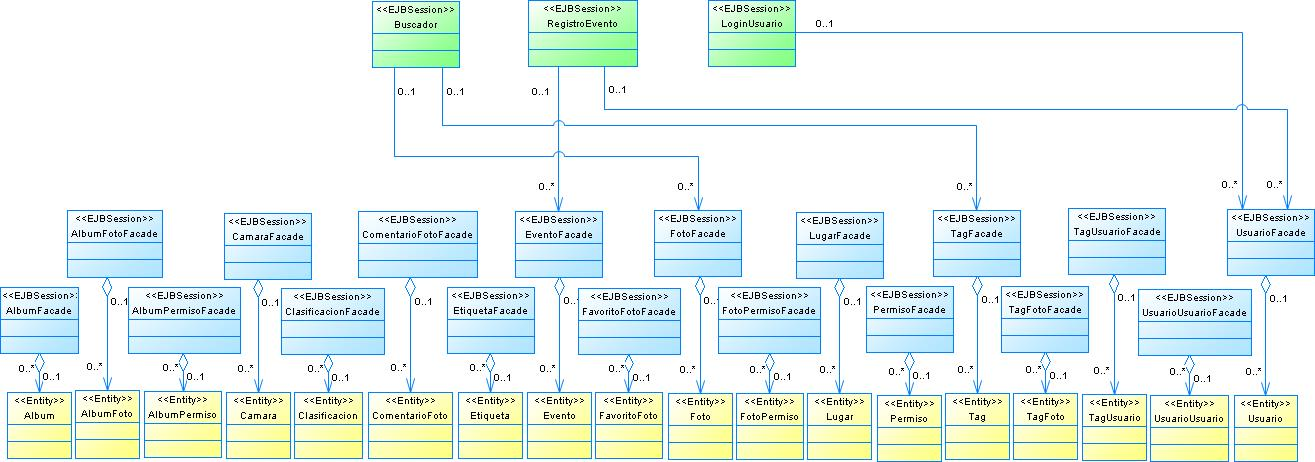
\includegraphics[width=17cm]{DiagramaModeloControlador.jpg}
}

El esquema general de las capas que se presentan en la imagen es: \textbf{Entidad - Facade - EJB Logical - Interface EJB - Service (Cadena 1)}.

\begin{itemize}
\item \textbf{Entidad}: : Corresponde a las clases entidades que permiten la comunicación con la base de datos. Estas entidades son utilizadas por las \textsl{Facade} para la persistencia de información de ser necesaria.

\item \textbf{Facade}: Heredan de \textsl{AbstractFacade} que entrega la estructura para los métodos que trabajan sobre las entidades. Los \textsl{Facades} entregan soporte a los \textsl{EJB Logical} para trabajar con la información de la base de datos y persistir esta.

\item \textbf{EJBLogical}: : Corresponden a la lógica de la aplicación, implementan los métodos necesarios para los servicios a entregar en el \textsl{web service}, se comunican con los \textsl{Facade} y con los diferentes \textsl{JAR} de \textsl{Lucene} y \textsl{Weka} para la implementación de los determinados servicios. Cada \textsl{EJBLogical} expone sus métodos para que los utilicen otros \textsl{EJBLogical} o los servicios mediante una interfaz (\textsl{Interface EJB}). 

\item \textbf{Interface EJB}: Existe uno por cada \textsl{EJBLigical}, y cada uno de los \textsl{EJBLogical} debe implementar todos los métodos definidos por la interfaz. Esta interfaz sirve para separar la lógica de los diferentes servicios que se pueden implementar.

\item \textbf{Service}: Son servicios que utilizan los diversos métodos entregados por las \textsl{Interface EJB} para generar los servicios pertinentes. Pueden utilizar más de un método y estos métodos pueden pertenecer a diversas interfaces. Utilizan los métodos propios de \textsl{HTTP} para entregar los servicios.
\end{itemize}

\figura{Diagrama de Clases JavaEE, parte 1).}{
	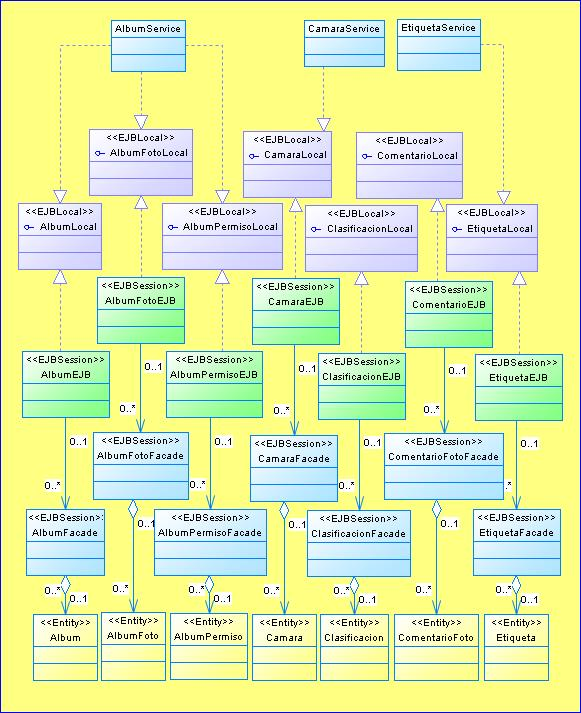
\includegraphics[width=11cm]{DiagramaModeloControladorParte1.jpg}
}

En la figura 2-2 se presenta la implementación necesaria para generar los servicios correspondientes a Album , Camara y Etiqueta. Como se aprecia el servicio correspondiente al álbum utiliza más de una interfaz con el fin de agrupar funcionalidades entregadas por la lógica de negocio para mejorar los servicios entregados. A su vez cada interfaz se comunica como lo señala la cadena 1.


\figura{Diagrama de Clases JavaEE, parte 2.}{
	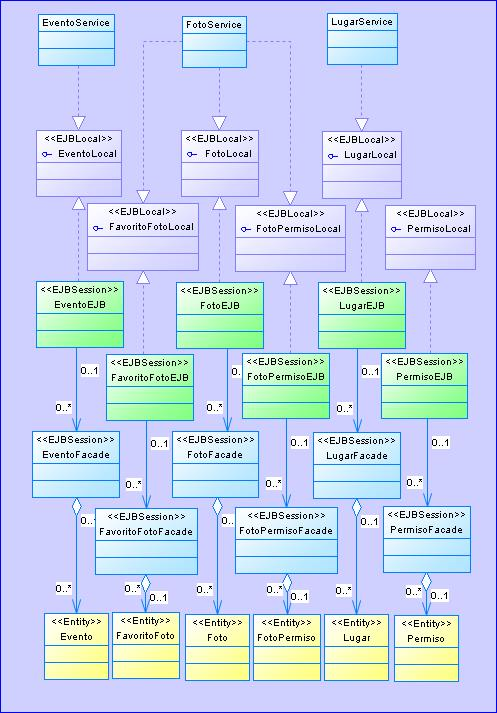
\includegraphics[width=11cm]{DiagramaModeloControladorParte2.jpg}
}

En la figura 2-3 se presenta la implementación necesaria para generar los servicios correspondientes a Evento , Foto y Lugar. Como se aprecia el servicio correspondiente a la foto utiliza más de una interfaz con el fin de agrupar funcionalidades entregadas por la lógica de negocio para mejorar los servicios entregados. A su vez cada interfaz se comunica como lo señala la cadena 1.

\figura{Diagrama de Clases JavaEE, parte 3.}{
	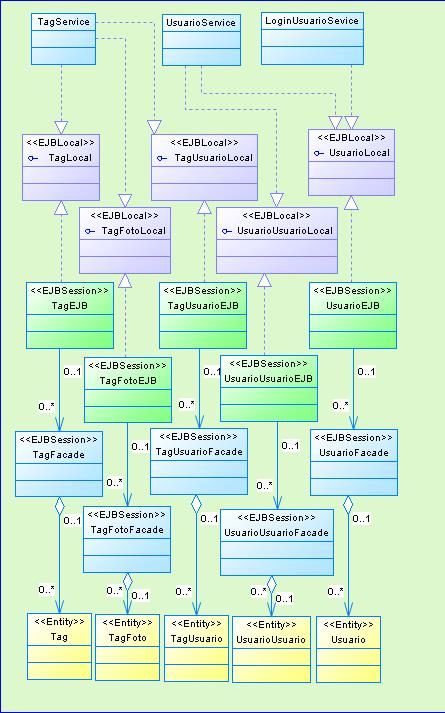
\includegraphics[width=11cm]{DiagramaModeloControladorParte3.jpg}
}

En la figura 2-4 se presenta la implementación necesaria para generar los servicios correspondientes a Tag , Usuario y Login. Como se aprecia los servicios correspondientes al Tag y Usuario, utiliza más de una interfaz con el fin de agrupar funcionalidades entregadas por la lógica de negocio para mejorar los servicios entregados. A su vez cada interfaz se comunica como lo señala la cadena 1.

\newpage
\subseccion{DIAGRAMA DE ENTITIES.}

A continuación se presenta el diagrama de clases correspondiente a la capa Modelo en MVC, donde se presenta la relación que existe entre clases de entidades (\textsl{Entity}), relaciones coherentes con las tablas mapeadas de la base de datos.

\figura{Diagrama de Clases JavaEE (Entities).}{
	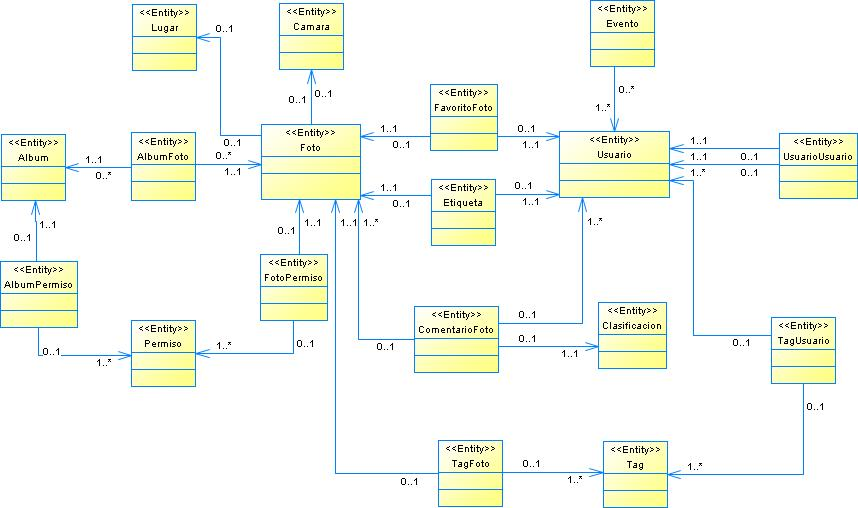
\includegraphics[width=16.5cm]{DiagramaEntities.jpg}
}

En la Figura 2-5, se observa la relación entre entidades. Las flechas indican asociación, indican que la entidad que tiene una punta de flecha es una llave foránea de la entidad que la conecta. Se aprecia que existe la entidad foto la cual junto con usuario forman parte de las entidades principales de la capa de modelo ya que existe una gran cantidad de entidades que utilizan las \textsl{primarykeys} de estas entidades como llaves foráneas.

\figura{Diagrama de Clases JavaEE (Entities), parte 1.}{
	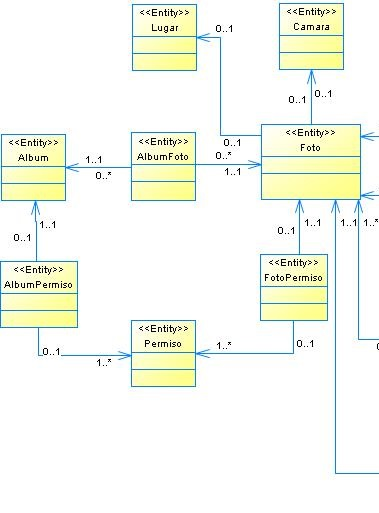
\includegraphics[width=10cm]{DiagramaEntitiesParte1.jpg}
}

Las entidades y relaciones mostradas en la figura 2-6 se detallan a continuación:

\begin{itemize}
\item Entidad \textbf{Cámara} se relaciona con la entidad \textbf{Foto}, con el fin de representar qué cámara se utilizó para la captura de la fotografía.
\item Entidad \textbf{Lugar} se relaciona con la entidad \textbf{Foto}, con el fin de señalar cuáles fueron los lugares en los cuales de tomo o localizó determinada fotografía.
\item Entidad \textbf{AlbumFoto} se relaciona con las entidades \textbf{Foto} y \textbf{Album}, con el fin de señalar que fotografías se encuentran en determinados álbumes.
\item Entidad \textbf{AlbumPermiso} y \textbf{FotoPermiso} se relacionan con las entidades \textbf{Foto} y \textbf{Álbum} respectivamente y ambas con la entidad Permiso, con el fin de entregar a las fotografías y álbumes del usuario un grado de permiso en el sistema.
\item Entidad \textbf{TagFoto} se relaciona con las entidades \textbf{Foto} y \textbf{Tag}, con el fin de representar que para una fotografía se puede utilizar determinado tag. Representa relación muchos a muchos entre \textbf{Foto} y \textbf{Tag}.
\end{itemize}

\figura{Diagrama de Clases JavaEE (Entities, parte 2).}{
	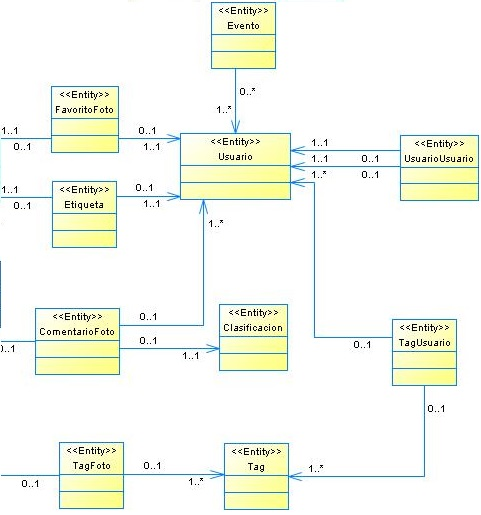
\includegraphics[width=11cm]{DiagramaEntitiesParte2.jpg}
}

Las entidades y relaciones mostradas en la figura 2-7 se detallan a continuación:

\begin{itemize}
\item Entidad \textbf{Evento} se relaciona con la entidad \textbf{Usuario}, con el fin de representar que cada usuario tendrá un historial de eventos en el sistema.
\item Entidad \textbf{UsuarioUsuario} se relaciona con la entidad \textbf{Usuario}, con el fin de representar cuando un usuario sigue a otro usuario de la aplicación con el objetivo de ver sus fotografías.
\item Entidad \textbf{TagUsuario} se relaciona con las entidades \textbf{Usuario} y \textbf{Tag}, con el fin de representar que un usuario puede utilizar más de un tag, \textbf{TagUsuario} se encarga de representar la relación muchos a muchos entre \textbf{Usuario} y \textbf{Tag}.
\item Entidad \textbf{ComentarioFoto} se relaciona con las entidades \textbf{Usuario} y \textbf{Foto}, con el fin de representar que un usuario puede comentar determinadas fotografías. A su vez representa la relación muchos a muchos entre \textbf{Foto} y \textbf{Usuario} enfocada a los comentarios que estos últimos realizan sobre las fotografías.
\item Entidad \textbf{Etiqueta} se relaciona con las entidades \textbf{Usuario} y \textbf{Foto}, con el fin de representar que un usuario puede ser etiquetado en determinada fotografía.
\item Entidad \textbf{Favorito} se relaciona con las entidades \textbf{Usuario} y \textbf{Foto}, con el fin de representar cuando un usuario agrega una fotografía a sus favoritas.
\end{itemize}

\newpage
\subseccion{DIAGRAMA DE BUSCADOR.}

A continuación se presenta el diagrama de clases correspondiente a la implementación del Buscador. Representado por la capa de Modelo - Controlador.

\figura{Diagrama de Clases Buscador.}{
	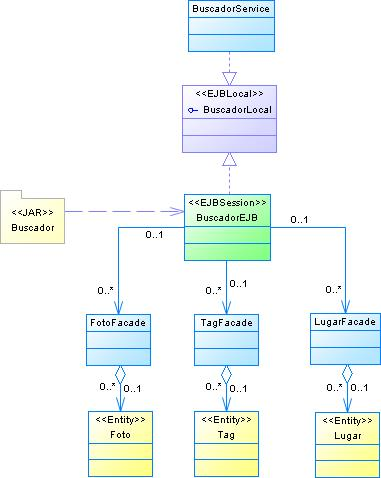
\includegraphics[width=11cm]{DiagramaBuscador.jpg}
}

Como se observa en la figura 2-8,  existe un servicio \textsl{BuscadorService} el cual mediante la biblioteca \textsl{javax.ws.rs} especializada en la creación de servicios \textsl{rest} mediante \textsl{EJBs}. Esta clase servicio se comunica con la interfaz local \textsl{BuscadorLocal}, que contiene los métodos para el buscador implementados por el \textsl{BuscadorEJB} que se comunica con el modelo mediante los \textsl{facade} correspondientes a la Foto, Tag y Lugar, además de comunicarse con el \textsl{Package} o \textsl{JAR} correspondiente a la implementación del buscador señalada en la sección 2.3.

\newpage
\seccion{DIAGRAMA WEB-APP (ANGULAR JS).}

\figura{Diagrama de Clases Angular JS.}{
	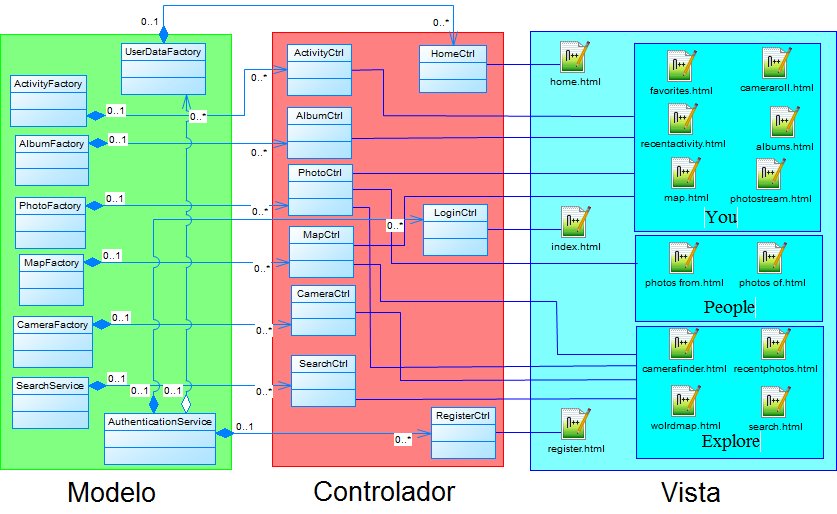
\includegraphics[width=17cm]{DiagramaClasesAngularJS.png}
}

El diagrama de clases en \textsl{AngularJS} tiene ciertas particularidades. Primero que todo, el diagrama está fuertemente influenciado por la Arquitectura \textsl{MVC} (Modelo-Vista-Controlador), además las estructuras de código en \textsl{AngularJS} no son clases en sí mismas, sino que son módulos que pueden cumplir diferentes propósitos según son definidos.

Dentro de los tipos de módulos tenemos los Controladores (encargados de intermediar las interacciones entre Modelo y Vista), las Factorías (encargadas de ofrecer objetos Javascript a través de funciones implementables) y los Servicios (encargados de recibir peticiones y procesarlas con la capa de Negocio).

Las Factorías y Servicios viven en la capa de Modelo, los Controladores viven en su capa homónima y los archivos HTML residen en la capa de Vista.

Cada vista HTML tiene un Controlador asignado, y cada Controlador puede llamar a una o más Factorías y Servicios, como se ve en la Figura del diagrama de clases de AngularJS.

La disposición de las clases está estrictamente ligado e impuesto por la arquitectura, en este sentido es una ventaja, ya que simplifica la tarea del diseño arquitectural a nivel de Aplicación Web.

\newpage
\seccion{DIAGRAMA LUCENE.}

El diagrama de clases mostrado en la figura 2-6, representa las principales clases que se utilizarán durante el desarrollo del buscador con la tecnología \textsl{Lucene}. Cabe mencionar que existen otras clases propias de la tecnología pero que para esta ocasión serán obviadas y solo se explicarán las principales y más características, tomando en cuenta que a medida que avance el proceso de implementación se puede utilizar muchas más clases.

\figura{Diagrama de Clases Lucene.}{	
	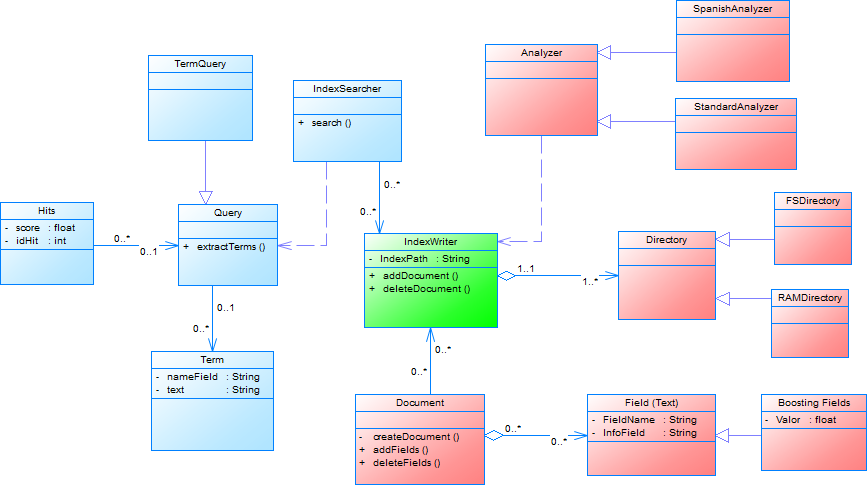
\includegraphics[width=17cm]{DiagramaClasesLucene.png}
}

Para comenzar, se muestra en la figura 2-7 la sección derecha del diagrama de la figura 2-6 que corresponde a las clases utilizadas en el proceso de indexación de \textsl{Lucene}. 

La clase \textsl{IndexWriter} (destacada con color verde en el diagrama) es la clase encargada de crear la estructura del índice invertido para realizar todas las búsquedas correspondientes. Se necesita de una clase \textsl{Analyzer}, con la que se analizarán los textos sobre los que se construirá el índice, dentro de esta clase, existen múltiples subclases de analizadores con distintos filtros, dentro de las cuales se encuentran las que se especificaron en el diagrama: \textsl{SpanishAnalyzer} y \textsl{StandardAnalyzer}, donde el primero sirve para trabajar con el lenguaje español, y el segundo se encarga de transformar todo a letra minúscula, de eliminar las \textsl{StopWords} y de aceptar caracteres especiales como acrónimos, alfanuméricos, entre otros.

Luego, se tiene una clase \textsl{Directory}, que es la encargada de almacenar el índice invertido que se ha creado. Dentro de esta clase se pueden encontrar dos subclases principales: \textsl{FSDirectory} y \textsl{RAMDirectory}. La primera, se encarga de almacenar el índice de manera física, es decir, se reserva un espacio de memoria en el disco duro donde se almacenará la estructura de datos, mientras que con \textsl{RAMDirectory} se almacena en memoria RAM para acceder de manera más rápida, luego de terminar los procesos de búsqueda, los índices en RAM se destruyen, no así los almacenados con la clase \textsl{FSDirectory}. 

\figura{Diagrama de Clases Lucene, parte 1.}{
	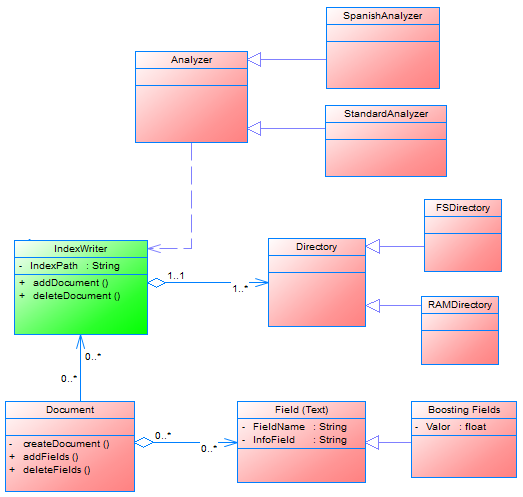
\includegraphics[width=15cm]{DiagramaClasesLuceneParte1.png}
}

Con la clase \textsl{Document}, se crean los diferentes documentos que contendrá el índice invertido, para esto, se utiliza la clase \textsl{Field}, que son los distintos campos que conformarán un documento. Cada campo, se clasifica de una manera diferente para establecer los valores que tendrán al momento de hacer una búsqueda, en este caso, se utilizará el campo \textsl{BoostingFields}, que indexarán los distintos campos asignándoles diferentes valores.
    
\newpage
\figura{Diagrama de Clases Lucene, parte 2.}{
	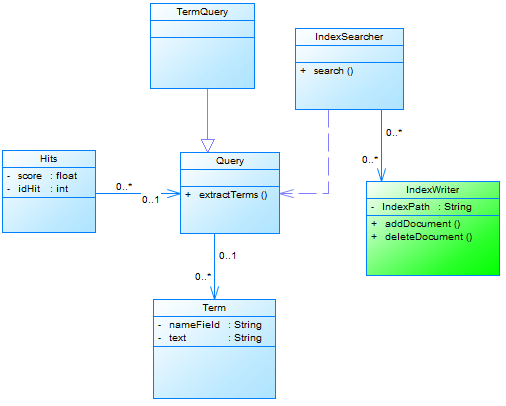
\includegraphics[width=15cm]{DiagramaClasesLuceneParte2.png}
}

Continuando con la sección izquierda del diagrama de clases, se pueden observar las clases que se utilizan para el proceso de búsqueda de \textsl{Lucene}. En primer lugar, se encuentra la clase \textsl{IndexSearcher} que se encarga de generar las búsquedas, encontrando los distintos índices invertidos (generados con \textsl{IndexWriter}) que participarán en una búsqueda específica. Dicha clase necesita de \textsl{Query}, que será la clase que realiza la consulta generada para encontrar los resultados esperados. Esta clase cuenta con varias subclases, entre ellas \textsl{TermQuery}, que es el \textsl{query} más básico y se usa para encontrar documentos con campos con valores específicos. La búsqueda como tal, debe utilizar la clase \textsl{Term}, que es la unidad básica para la búsqueda, conteniendo el nombre del \textsl{field} y el valor que se le asigna (con la clase \textsl{Boosting Fields} explicada anteriormente). Y por último, se encuentra la clase \textsl{Hit}, en donde se almacenarán todos los resultados de documentos encontrados relacionados con la búsqueda del \textsl{Query}. 

\newpage
\seccion{DIAGRAMA ANDROID.}

En el siguiente diagrama, se muestran las clases que se deberán implementar para la aplicación en el sistema operativo \textsl{Android}.

\figura{Diagrama de Clases Android.}{
	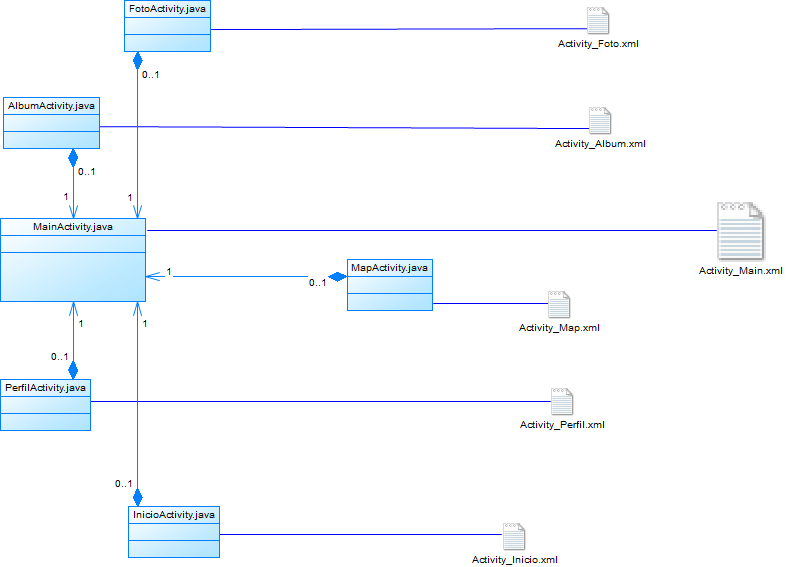
\includegraphics[width=18cm]{DiagramaClasesAndroid.png}
}

Al observar el diagrama presentado en la figura 2-9, se puede observar que existen dos tipos de archivos, estos son los \textsl{.java} y \textsl{.xml}. Los primeros son clases o \textsl{Activitys}, estos en \textsl{Android} son las pantallas que se presentan al usuario; \textsl{MainActivity} representa la primera pantalla que se muestra en donde el usuario debe iniciar sesión para entrar  a la aplicación. De esta \textsl{Activity} se desprenden las demás vistas a las que se puede entrar, como por ejemplo la \textsl{Activity} de nombre \textsl{InicioActivity} es donde ingresa el usuario luego de ser verificado por el sistema, aquí el usuario puede ver las actividades recientes de contactos y las fotos subidas por éstos, en esta vista el usuario tiene la opción para desplazarse por las demás \textsl{Activitys} disponibles. Existe una \textsl{Activity} para cuando el usuario quiera subir una foto, esta es \textsl{FotoActivity}, en donde el usuario puede seleccionar la imagen a subir al sistema y editar la información de ésta. En \textsl{AlbumActivity} el usuario puede visualizar los álbumes que tiene en su cuenta y las fotos que componen a éstos. También existe la vista de \textsl{PerfilActivity} que se utiliza para visualizar el perfil del usuario en la sesión actual. Por último, para las foto geo-localizadas está la \textsl{MapActivity}, que muestra al usuario el mapa mundial de fotos con sus distintas fotografías que han sido localizadas. En el diagrama se observa una dependencia de todas estas clases a \textsl{MainActivity}, ya que es esta la que inicia la aplicación y las demás no pueden existir sin que ésta exista, por esa razón las cardinalidades asociadas a cada una de las relaciones. 

El segundo tipo de archivos que se observa son los \textsl{.xml}, éstos son los \textsl{Layout} de la aplicación y es donde se diseña la vista para que sea visualizada por el usuario. Cada una de las \textsl{Activitys} anteriormente mencionadas cuenta con su archivo de vista respectivo como se puede apreciar en el diagrama. Éstos son los archivos con los que interactúa el usuario al observar la aplicación, pero las clases o \textsl{Activitys} mencionadas son las que realizan las acciones que el usuario comanda.
 
%-------------------------------------------------------------------------------------
\capitulo{CASOS DE USO.}

A continuación, se detallan todos los casos de uso que se especificaron en una entrega anterior (Entrega 1: Ingeniería de Requerimientos), donde se desarrolló el siguiente diagrama:

\figura{Diagrama de Casos de Uso (Ingeniería de Requerimientos.}{
	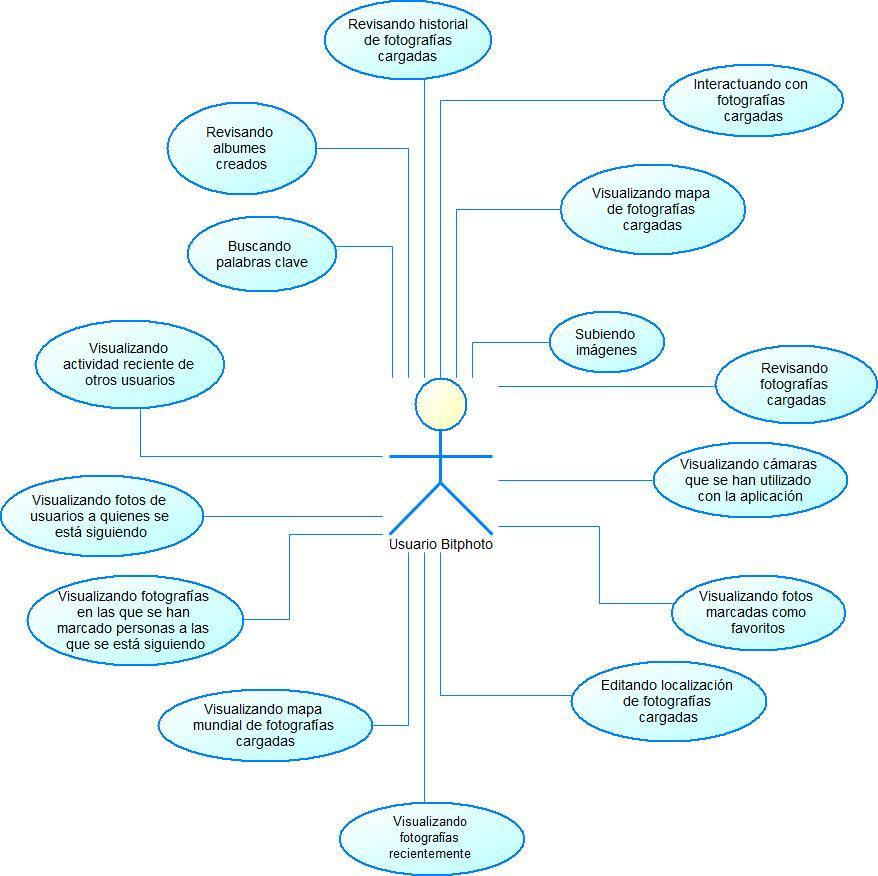
\includegraphics[width=16.5cm]{DiagramaDeCasosDeUso.jpg}
}

\newpage
\tabla{Caso de Uso CU01: Revisando historial de fotografías cargadas.}{
	\begin{tabular}[c]{|p{2.7cm}|p{13.3cm}|}
		\hline
		\textbf{ID}  & CU01\\ \hline
		\textbf{Nombre} & Revisando historial de fotografías cargadas\\ \hline
		\textbf{Resumen} & El usuario puede ver sus fotografías cargadas al sistema, agrupadas por la fecha en que fueron tomadas o subidas a la aplicación.\\ \hline
		\textbf{Actores} & Usuario\\ \hline
		\textbf{Precondiciones} & El usuario inicia sesión en el sistema ingresando cuenta y contraseña válidas.\\ \hline
		\textbf{Descripción} & El usuario, luego de iniciar sesión y encontrarse en la página principal del sistema, selecciona la opción “Camera Roll”. Luego de encontrarse en la vista “Camera Roll”, se muestran todas las fotografías que ha subido el usuario a la aplicación agrupadas la fecha en que fueron subidas a la plataforma, luego selecciona la opción “fecha de toma”, luego se muestra la vista “Camera Roll” con las fotografías del usuario agrupadas por la fecha en que fueron tomadas por el usuario. (EX01: El usuario no ha subido fotografías a la aplicación). Luego, el usuario selecciona cualquiera de las fotografías que se muestran para revisar toda la información asociada, como los comentarios, cantidad de favoritos, entre otras.\\ \hline
		\textbf{Postcondiciones} & El usuario se encuentra en la vista “Camera Roll” visualizando las fotografias propias subidas a la aplicación, permitiéndole escoger cualquiera de ellas para revisar su información.\\ \hline
		\textbf{Requisitos de Usabilidad} & El sistema indica al usuario que se encuentra en la vista “Camera Roll” mediante un título o un encabezado en la página.\\ \hline
		\textbf{Excepciones} & \textbf{Ex01: El usuario no ha subido fotografías a la aplicación.}
		
Puede suceder que el usuario aún no suba fotografías a la aplicación, por lo tanto, se le informará por pantalla que no ha subido fotografías a la aplicación.
\\ \hline
	\end{tabular}
}

\newpage
\tabla{Caso de Uso CU02: Revisando fotografías cargadas.}{
	\begin{tabular}[c]{|p{2.7cm}|p{13.3cm}|}
		\hline
		\textbf{ID}  & CU02\\ \hline
		\textbf{Nombre} & Revisando fotografías cargadas\\ \hline
		\textbf{Resumen} & El usuario puede ver las fotografías que ha subido a la aplicación ordenadas por fechas en que fueron subidas o fecha en que fueron tomadas.\\ \hline
		\textbf{Actores} & Usuario\\ \hline
		\textbf{Precondiciones} & El usuario inicia sesión en el sistema ingresando cuenta y contraseña válidas.\\ \hline
		\textbf{Descripción} & El usuario, luego de iniciar sesión y encontrarse en la página principal del sistema, selecciona la opción “Photostream”. Luego de encontrarse en la vista “Photostream”, se muestran las fotografías del usuario ordenadas por la fecha en que fueron subidas a la aplicación. (EX01: No existen fotografías del usuarios). A continuación el usuario selecciona la opción “fecha de toma”, ahora en la vista “photostream” se muestran las fotos del usuario ordenadas por la fecha en fueron tomas.(EX01: No existen fotografías del usuarios). Luego, el usuario selecciona cualquiera de las fotografías que se muestran para revisar toda la información asociada, como los comentarios, cantidad de favoritos, entre otras.\\ \hline
		\textbf{Postcondiciones} & El usuario se encuentra en la vista “photostream” visualizando todas las fotografías de otros usuarios, permitiéndole escoger cualquiera de ellas para revisar su información.\\ \hline
		\textbf{Requisitos de Usabilidad} & El sistema indica al usuario que se encuentra en la vista “Photostream” mediante un título o un encabezado en la página.\\ \hline
		\textbf{Excepciones} & \textbf{Ex01: No existen fotografías del usuario.}

Puede suceder que el usuario aún no suba fotografías a la aplicación, por lo tanto, se le informará por pantalla que no ha subido fotografías a la aplicación. 
\\ \hline
	\end{tabular}
}

\newpage
\tabla{Caso de Uso CU03: Revisando álbumes creados.}{
	\begin{tabular}[c]{|p{2.7cm}|p{13.3cm}|}
		\hline
		\textbf{ID}  & CU03\\ \hline
		\textbf{Nombre} & Revisando álbumes creados\\ \hline
		\textbf{Resumen} & El usuario puede ver los álbumes que ha creado en el sistema, además puede ver qué fotografías se encuentran en cada álbum.\\ \hline
		\textbf{Actores} & Usuario\\ \hline
		\textbf{Precondiciones} & El usuario inicia sesión en el sistema ingresando cuenta y contraseña válidas.\\ \hline
		\textbf{Descripción} & El usuario, luego de iniciar sesión y encontrarse en la página principal del sistema, selecciona la opción “Álbumes”. Luego de encontrarse en la vista “Álbumes”, se muestran los álbumes que el usuario a creado.(EX01: El usuario no ha creado ningún álbum). El usuario selecciona un álbum, luego se muestra en la vista “Álbumes” las fotografías contenidas en este. Luego, el usuario selecciona cualquiera de las fotografías que se muestran para revisar toda la información asociada, como los comentarios, cantidad de favoritos, entre otras.\\ \hline
		\textbf{Postcondiciones} & El usuario se encuentra en la vista “Álbumes” visualizando los álbumes creados, permitiéndole escoger un álbum y revisar que fotográficas contiene, además de permitirle seleccionar cualquier fotografía para poder revisar su información.\\ \hline
		\textbf{Requisitos de Usabilidad} & El sistema indica al usuario que se encuentra en la vista “Álbumes” mediante un título o un encabezado en la página.\\ \hline
		\textbf{Excepciones} & \textbf{Ex01: El usuario no ha creado ningún álbum.}

Existe la posibilidad de que el usuario no haya creado ningún álbum, en este caso, se le informa que no existen álbumes.
\\ \hline
	\end{tabular}
}

\newpage
\tabla{Caso de Uso CU04: Visualizando mapa de fotografías cargadas.}{
	\begin{tabular}[c]{|p{2.7cm}|p{13.3cm}|}
		\hline
		\textbf{ID}  & CU04\\ \hline
		\textbf{Nombre} & Visualizando mapa de fotografías cargadas\\ \hline
		\textbf{Resumen} & El usuario podrá visualizar un mapa en el que ha localizado las fotografías que ha cargado a la aplicación.\\ \hline
		\textbf{Actores} & Usuario\\ \hline
		\textbf{Precondiciones} & El usuario inicia sesión en el sistema ingresando cuenta y contraseña válidas.\\ \hline
		\textbf{Descripción} & El usuario, luego de iniciar sesión y encontrarse en la página principal del sistema, selecciona la opción “Mapa”. Luego de encontrarse en la vista “Mapa”, se muestra un mapa donde el usuario ha localizado las fotografías que ha cargado a la aplicación, mostrándose la ubicación con un punto (EX01: El usuario no ha localizado ninguna fotografía.). Posteriormente el usuario selecciona cualquiera de las fotografías encontradas en el mapa para observar toda la información que esté asociada a ésta (comentarios, personas marcadas, entre otros).  \\ \hline
		\textbf{Postcondiciones} & El usuario se encuentra en la vista “Mapa” visualizando las fotografías localizadas. \\ \hline
		\textbf{Requisitos de Usabilidad} & El sistema indica al usuario que se encuentra en la vista “Mapa” mediante un título o un encabezado en la página.\\ \hline
		\textbf{Excepciones} & \textbf{Ex01: El usuario no ha localizado ninguna fotografía.}

Si el usuario no ha asignado ninguna ubicación a las fotografías que ha cargado a la página, el mapa se mostrará de igual manera informándole a través de un mensaje que no ha localizado ninguna fotografía.
\\ \hline
	\end{tabular}
}

\newpage
\tabla{Caso de Uso CU05: Editanto localización de fotografías cargadas.}{
	\begin{tabular}[c]{|p{2.7cm}|p{13.3cm}|}
		\hline
		\textbf{ID}  & CU05\\ \hline
		\textbf{Nombre} & Editanto localización de fotografías cargadas\\ \hline
		\textbf{Resumen} & El usuario puede editar la localización de las fotografías que ha cargado en la aplicación.\\ \hline
		\textbf{Actores} & Usuario\\ \hline
		\textbf{Precondiciones} & El usuario inicia sesión en el sistema ingresando cuenta y contraseña válidas.\\ \hline
		\textbf{Descripción} & El usuario, luego de iniciar sesión y encontrarse en la página principal del sistema, selecciona la opción “Editar Fotografía”. Luego de encontrarse en la vista “Editar Fotografía”, selecciona la opción “Editar Ubicación”, correspondiente a la opción para cambiar la localización de la fotografía en el mapa. Posteriormente el usuario ingresa el nombre del país en el que desea ubicar la fotografía (EX01: El país ingresado no es válido) y finaliza la edición. Por último, se mostrará en el mapa el país al que ha sido asociada la fotografía y éste aparecerá en la información al momento de revisar la misma.\\ \hline
		\textbf{Postcondiciones} & El usuario se encuentra en la vista “Editar Fotografía” donde aparecen todas las opciones de edición dentro de las que se muestra “Editar Ubicación”.\\ \hline
		\textbf{Requisitos de Usabilidad} & El sistema indica al usuario que se encuentra en la vista “Editar Fotografía” mediante un título o un encabezado en la página.\\ \hline
		\textbf{Excepciones} & \textbf{Ex01: El país ingresado no es válido.}
		
Puede suceder que el usuario, al momento de ingresar el país en el que desea ubicar la fotografía, ingrese el nombre mal escrito, o ingrese números u otros caracteres no válidos, en este caso se le muestra un mensaje de alerta informándole del error y solicitando que ingrese el nombre nuevamente.
\\ \hline
	\end{tabular}
}

\newpage
\tabla{Caso de Uso CU06: Visualizando fotografías marcadas como favoritos.}{
	\begin{tabular}[c]{|p{2.7cm}|p{13.3cm}|}
		\hline
		\textbf{ID}  & CU06\\ \hline
		\textbf{Nombre} & Visualizando fotografías marcadas como favoritos\\ \hline
		\textbf{Resumen} & El usuario puede ver las fotografías en las que ha marcado la opción “favoritos”.\\ \hline
		\textbf{Actores} & Usuario\\ \hline
		\textbf{Precondiciones} & El usuario inicia sesión en el sistema ingresando cuenta y contraseña válidas.\\ \hline
		\textbf{Descripción} & El usuario, luego de iniciar sesión puede revisar la información asociada de cualquier fotografía en las vistas correspondientes (vista “Explorar”, en el perfil de un amigo, mapa del mundo, entre otras) y marcar la opción “Favorito” si es que lo desea. Luego, todas las fotografías en las que haya marcado esta opción, se encontrarán en la vista “Favoritos”, donde el usuario puede revisar la información asociada en cualquier momento. \\ \hline
		\textbf{Postcondiciones} & El usuario se encuentra en la vista “Favoritos” visualizando todas las fotografías en las que se ha marcado la opción “Favorito”.\\ \hline
		\textbf{Requisitos de Usabilidad} & El sistema indica al usuario que se encuentra en la vista “Favoritos” mediante un título o un encabezado en la página.\\ \hline
		\textbf{Excepciones} & \\ \hline
	\end{tabular}
}

\newpage
\tabla{Caso de Uso CU07: Visualizando actividad reciente de otros usuarios.}{
	\begin{tabular}[c]{|p{2.7cm}|p{13.3cm}|}
		\hline
		\textbf{ID}  & CU07\\ \hline
		\textbf{Nombre} & Visualizando actividad reciente de otros usuarios\\ \hline
		\textbf{Resumen} & El usuario puede ver la actividad reciente de otros usuarios relacionadas con él mismo (ya sea en las fotografías del usuario, respuestas a los comentarios del usuario, entre otros).\\ \hline
		\textbf{Actores} & Usuario\\ \hline
		\textbf{Precondiciones} & El usuario inicia sesión en el sistema ingresando cuenta y contraseña válidas.\\ \hline
		\textbf{Descripción} & El usuario, luego de iniciar sesión y encontrarse en la página principal del sistema, selecciona la opción “Actividad Reciente”. Luego de encontrarse en la vista “Actividad Reciente”, se muestra toda actividad de otras personas que esté relacionada con el usuario, por ejemplo, respuesta a sus comentarios, actividad en las fotografías que ha cargado al sistema, nuevos seguidores, entre otras (EX01: No existe actividad reciente de otros usuarios).  \\ \hline
		\textbf{Postcondiciones} & El usuario se encuentra en la vista “Actividad Reciente” visualizando toda la actividad de otros usuarios. \\ \hline
		\textbf{Requisitos de Usabilidad} & El sistema indica al usuario que se encuentra en la vista “Actividad Reciente” mediante un título o un encabezado en la página.\\ \hline
		\textbf{Excepciones} & \textbf{Ex01: No existen actividad reciente de otros usuarios.}
		
Puede suceder que no existan actividades de otras personas relacionadas con el usuario, por lo tanto, se le informará por pantalla que no ha habido interacciones.
\\ \hline
	\end{tabular}
}

\newpage
\tabla{Caso de Uso CU08: Viendo fotografías de usuarios a quienes se sigue.}{
	\begin{tabular}[c]{|p{2.7cm}|p{13.3cm}|}
		\hline
		\textbf{ID}  & CU08\\ \hline
		\textbf{Nombre} & Visualizando fotografías de usuarios a quienes se está siguiendo\\ \hline
		\textbf{Resumen} & El usuario puede ver las fotografías de las personas que está siguiendo escogiendo entre ver 1 o 5 fotografías por persona.\\ \hline
		\textbf{Actores} & Usuario\\ \hline
		\textbf{Precondiciones} & El usuario inicia sesión en el sistema ingresando cuenta y contraseña válidas.\\ \hline
		\textbf{Descripción} & El usuario, luego de iniciar sesión y encontrarse en la página principal del sistema, selecciona la opción “Fotos de”. Luego de encontrarse en la vista “Fotos de”, se muestran las fotografías de las personas a las que está siguiendo (EX01: No hay fotografías de otros usuarios). Dependiendo del filtro de la cantidad de fotografías que el usuario escoja, verá 1 o 5 fotografías por cada persona que está siguiendo (EX02: Uno o más usuarios tiene menos de 5 fotografías). Luego, el usuario selecciona cualquier fotografía que se muestre para ver toda la información asociada, como comentarios, cantidad de favoritos, entre otras.\\ \hline
		\textbf{Postcondiciones} & El usuario se encuentra en la vista “Fotos de” viendo todas las fotografías de otros usuarios, permitiéndole escoger cualquiera para ver la información.\\ \hline
		\textbf{Requisitos de Usabilidad} & El sistema indica al usuario que se encuentra en la vista “Fotos de” mediante un título o un encabezado en la página.\\ \hline
		\textbf{Excepciones} & \textbf{Ex01: No hay fotografías de otros usuarios.}
		
Es posible que el usuario esté siguiendo solamente a personas que no hayan subido ninguna fotografía, en este caso, se le informa que las personas que sigue no han subido fotografías y se le recomienda seguir a otros usuarios.

\textbf{Ex02: Uno o más usuarios tiene menos de 5 fotografías.}

En caso que el usuario desee ver 5 fotografías por persona y haya una o más personas que no tengan esa cantidad de fotografías cargadas, de igual forma se hace el filtro correspondiente y se muestran las fotografías que tengan (por ejemplo, si un usuario solo tiene 3 fotografías, se hace el filtro por 5 y solo se muestran las que se han cargado).  
\\ \hline
	\end{tabular}
}

\newpage
\tabla{Caso de Uso CU09: Visualizando fotografías en las que se han marcado personas a las que se está siguiendo.}{
	\begin{tabular}[c]{|p{2.7cm}|p{13.3cm}|}
		\hline
		\textbf{ID}  & CU09\\ \hline
		\textbf{Nombre} & Visualizando fotografías en las que se han marcado personas a las que se está siguiendo\\ \hline
		\textbf{Resumen} & El usuario puede ver las fotografías de cualquier persona, en las que se ha marcado a otros usuarios que está siguiendo.\\ \hline
		\textbf{Actores} & Usuario\\ \hline
		\textbf{Precondiciones} & El usuario inicia sesión en el sistema ingresando cuenta y contraseña válidas.\\ \hline
		\textbf{Descripción} & El usuario, luego de iniciar sesión y encontrarse en la página principal del sistema, selecciona la opción “Fotos con”. Luego de encontrarse en la vista “Fotos con”, se muestran las fotografías en las se ha marcado a personas a las que está siguiendo (EX01: Ninguna persona a la que sigue el usuario se ha marcado en alguna fotografía). Las fotografías en la que se han marcado las personas a las que el usuario sigue pueden ser de cualquier persona, incluso personas que no está siguiendo. Luego, el usuario selecciona cualquiera de las fotografías que se muestran para revisar toda la información asociada, como los comentarios, cantidad de favoritos, entre otras.\\ \hline
		\textbf{Postcondiciones} & El usuario se encuentra en la vista “Fotos con” visualizando todas las fotografías en las que se ha marcado a otros usuarios, permitiéndole escoger cualquiera de ellas para revisar la información.\\ \hline
		\textbf{Requisitos de Usabilidad} & El sistema indica al usuario que se encuentra en la vista “Fotos con” mediante un título o un encabezado en la página.\\ \hline
		\textbf{Excepciones} & \textbf{Ex01: Ninguna persona a la que sigue el usuario se ha marcado en alguna fotografía.}
		
Existe la posibilidad que no se marque en ninguna fotografía a ninguna de las personas que el usuario está siguiendo, en este caso, se le informa que no existen dichas fotografías.
\\ \hline
	\end{tabular}
}

\newpage
\tabla{Caso de Uso CU10: Visualizando fotografías recientemente cargadas a la aplicación.}{
	\begin{tabular}[c]{|p{2.7cm}|p{13.3cm}|}
		\hline
		\textbf{ID}  & CU10\\ \hline
		\textbf{Nombre} & Visualizando fotografías recientemente cargadas a la aplicación\\ \hline
		\textbf{Resumen} & El usuario podrá ver una fotografía de las que se han subido recientemente a la aplicación por todos los usuarios de ésta.\\ \hline
		\textbf{Actores} & Usuario\\ \hline
		\textbf{Precondiciones} & El usuario inicia sesión en el sistema ingresando cuenta y contraseña válidas.\\ \hline
		\textbf{Descripción} & El usuario selecciona la opción fotos recientes, donde el sistema muestra en la vista correspondiente las fotografías filtradas, el usuario selecciona una de éstas fotografías, por lo que el sistema responde mostrando solo ésta, junto con sus comentarios, descripción, fecha de carga y cantidad de favoritos según corresponda.\\ \hline
		\textbf{Postcondiciones} & El sistema muestra una fotografía en detalle.\\ \hline
		\textbf{Requisitos de Usabilidad} & El sistema indica al usuario que se encuentra en la vista “Fotos Recientes” mediante un título o un encabezado en la página.\\ \hline
		\textbf{Excepciones} & \\ \hline
	\end{tabular}
}

\newpage
\tabla{Caso de Uso CU11: Visualizando mapa mundial de fotografías cargadas.}{
	\begin{tabular}[c]{|p{2.7cm}|p{13.3cm}|}
		\hline
		\textbf{ID}  & CU11\\ \hline
		\textbf{Nombre} & Visualizando mapa mundial de fotografías cargadas\\ \hline
		\textbf{Resumen} & El usuario puede ver fotografías que se encuentran en un país a seleccionar en el mapa.\\ \hline
		\textbf{Actores} & Usuario\\ \hline
		\textbf{Precondiciones} & El usuario inicia sesión en el sistema ingresando cuenta y contraseña válidas.\\ \hline
		\textbf{Descripción} & El usuario debe seleccionar la opción mapa mundial, por lo que el sistema responde cargando en una vista el mapa correspondiente, donde el usuario procede a seleccionar un país en el cual desea buscar fotografías, por lo que el sistema carga las imágenes ubicadas en el país correspondiente (Ex 1: No existen fotografías asociadas con la ubicación).\\ \hline
		\textbf{Postcondiciones} & El sistema carga las fotografías asociadas a la ubicación seleccionada.\\ \hline
		\textbf{Requisitos de Usabilidad} & El sistema indica al usuario que se encuentra en la vista “Mapa del Mundo” mediante un título o un encabezado en la página.\\ \hline
		\textbf{Excepciones} & \textbf{Ex01: No existen fotografías asociadas a la ubicación.}
		
El sistema avisa al usuario que la ubicación seleccionada no tiene fotografías asociadas.
\\ \hline
	\end{tabular}
}

\newpage
\tabla{Caso de Uso CU12: Visualizando cámaras que se han utilizado con la aplicación.}{
	\begin{tabular}[c]{|p{2.7cm}|p{13.3cm}|}
		\hline
		\textbf{ID}  & CU12\\ \hline
		\textbf{Nombre} & Visualizando cámaras que se han utilizado con la aplicación\\ \hline
		\textbf{Resumen} & El usuario puede ver las cámaras y sus características correspondientemente. \\ \hline
		\textbf{Actores} & Usuario\\ \hline
		\textbf{Precondiciones} & El usuario inicia sesión en el sistema ingresando cuenta y contraseña válidas.\\ \hline
		\textbf{Descripción} & El usuario selecciona la opción cámaras, por lo que el sistema carga éstas y muestra un ranking de las cámaras más utilizadas en la aplicación, luego el usuario selecciona una de las cámaras, así el sistema muestra las características de la cámara seleccionada.\\ \hline
		\textbf{Postcondiciones} & El sistema carga en una vista las características de la cámara específicamente seleccionada.\\ \hline
		\textbf{Requisitos de Usabilidad} & El sistema indica al usuario que se encuentra en la vista “Buscador de Cámaras” mediante un título o un encabezado en la página.\\ \hline
		\textbf{Excepciones} & \\ \hline
	\end{tabular}
}

\newpage
\tabla{Caso de Uso CU13: Buscando palabra clave.}{
	\begin{tabular}[c]{|p{2.7cm}|p{13.3cm}|}
		\hline
		\textbf{ID}  & CU13\\ \hline
		\textbf{Nombre} & Buscando palabra clave\\ \hline
		\textbf{Resumen} & El usuario puede buscar una palabra clave en la sección del buscador (ya sea para encontrar fotografías con la palabra en tags, en el nombre, descripción o comentarios o otros usuarios que contengan la palabra en su nombre de usuario).\\ \hline
		\textbf{Actores} & Usuario\\ \hline
		\textbf{Precondiciones} & El usuario inicia sesión en el sistema ingresando cuenta y contraseña válidas.\\ \hline
		\textbf{Descripción} & El usuario, luego de iniciar sesión y encontrarse en la página principal del sistema, escribe una o más palabras en el buscador y luego selecciona buscar, al encontrarse en la vista “Buscador” este muestra todas las coincidencias con la o las palabras claves insertadas por el usuario(EX01: no existen coincidencias con la búsqueda realizada).  \\ \hline
		\textbf{Postcondiciones} & El usuario se encuentra en la vista “Busqueda”, visualizando las coincidencias encontradas por el buscador.\\ \hline
		\textbf{Requisitos de Usabilidad} & El sistema indica al usuario que se encuentra en la vista “Busqueda” mediante un título o un encabezado en la página.\\ \hline
		\textbf{Excepciones} & \textbf{Ex01: No existen coincidencias con la búsqueda realizada.}
		
Puede suceder que no existan coincidencias de búsqueda con la o palabras claves ingresadas, en ese caso el sistema informara que no se pudo encontrar nada con la información recibida.
\\ \hline
	\end{tabular}
}

\newpage
\tabla{Caso de Uso CU14: Subiendo imágenes.}{
	\begin{tabular}[c]{|p{2.7cm}|p{13.3cm}|}
		\hline
		\textbf{ID}  & CU14\\ \hline
		\textbf{Nombre} & Subiendo imágenes\\ \hline
		\textbf{Resumen} & El usuario sube imagen y edita sus campos(Agregar descripción, tags, personas, etc).\\ \hline
		\textbf{Actores} & Usuario\\ \hline
		\textbf{Precondiciones} & El usuario inicia sesión en el sistema ingresando cuenta y contraseña válidas.\\ \hline
		\textbf{Descripción} & El usuario, luego de iniciar sesión y encontrarse en la página principal del sistema, selecciona la opción “Subir foto”. Luego de encontrarse en la vista “Subir foto”, se muestran las opciones que puede llenar, para la información de la fotografía.(EX01: No existe una fotografía para subir o no es del formato valido). El usuario rellena los distintos campos de la información de la fotografía y selecciona “Subir foto”.\\ \hline
		\textbf{Postcondiciones} & El usuario se puede visualizar la fotografía recientemente subida al sistema.\\ \hline
		\textbf{Requisitos de Usabilidad} & El sistema indica al usuario que se encuentra en la vista “Subir foto” mediante un título o un encabezado en la página.\\ \hline
		\textbf{Excepciones} & \textbf{Ex01: No existe una fotografía para subir.}
		
El usuario no ha seleccionado una fotografía para subir al sistema, el sistema le indica por pantalla que no ha seleccionado una fotografía o que esta no es válida para subir, ya sea por el formato u otro problema, para esto el usuario debe seleccionar una fotografía valida para editar y subir al sistema.
\\ \hline
	\end{tabular}
}

\newpage
\tabla{Caso de Uso CU15: Interactuando con fotografías cargadas.}{
	\begin{tabular}[c]{|p{2.7cm}|p{13.3cm}|}
		\hline
		\textbf{ID}  & CU15\\ \hline
		\textbf{Nombre} & Interactuando con fotografías cargadas\\ \hline
		\textbf{Resumen} & El usuario puede ver la información de alguna  fotografía cargada y agregar información a esta fotografía (ya sea agregar comentario, marcar como favorito, agregar personas, etc).\\ \hline
		\textbf{Actores} & Usuario\\ \hline
		\textbf{Precondiciones} & El usuario inicia sesión en el sistema ingresando cuenta y contraseña válidas.\\ \hline
		\textbf{Descripción} & El usuario, luego de iniciar sesión y encontrarse en la página principal del sistema, selecciona la fotografía que quiere visualizar, el usuario interactúa con la fotografía (Agregando comentario, marcando como favorito, agregando personar, agregando tags), luego el sistema guarda los cambios y de la fotografía y se encuentra nuevamente visualizando la fotografía con la información agregada realizados.\\ \hline
		\textbf{Postcondiciones} & El usuario se encuentra en la vista visualizando la foto con la que realizo una interacción y puede observar la interaccione realizada, que cambio alguna información de la fotografía.\\ \hline
		\textbf{Requisitos de Usabilidad} & El sistema indica al usuario el cambio que se realiza en la fotografía.\\ \hline
		\textbf{Excepciones} & \\ \hline
	\end{tabular}
}


%-------------------------------------------------------------------------------------
\capitulo{DIAGRAMAS DE SECUENCIA.}

A continuación se presentan los diagramas de secuencia correspondientes a las implementaciones realizadas para esta entrega que son Visualizando Álbumes del Usuario y Visualizando Fotos del Usuario.

\seccion{Visualizando Fotos Usuario.}

\figura{Diagrama de Secuencia: Visualizando Fotografías Usuario.}{
	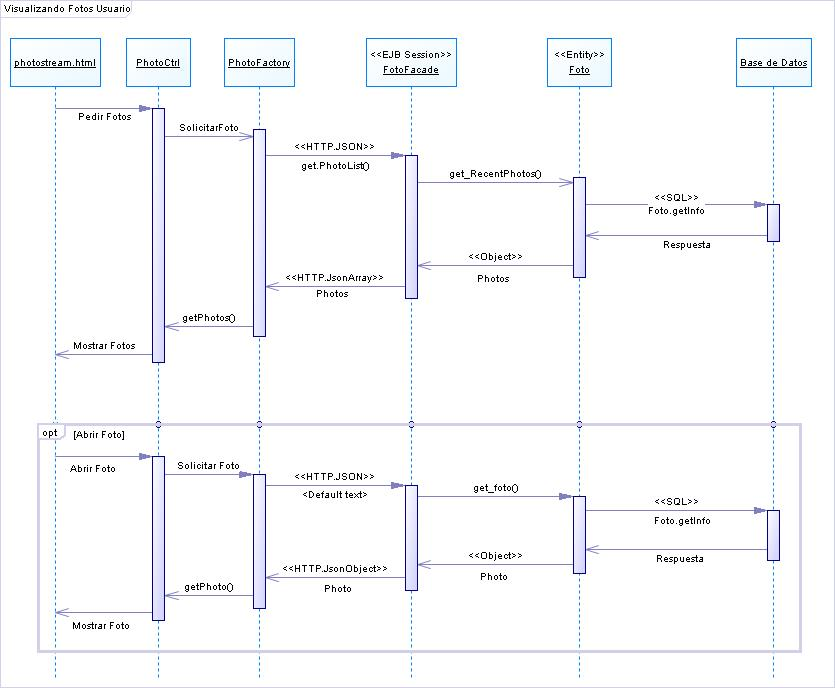
\includegraphics[width=17cm]{DiagramaSecuenciaPhotostream.jpg}
}

En este diagrama de secuencia se busca mostrar el comportamiento del sistema ante eventuales acciones por parte del usuario, en este caso el usuario se encuentra en primera instancia en la vista \textsl{PhotoSteam}, luego al cargar la página en el navegador se recibe la petición desde la vista y se procesa gracias a \textsl{angularJS} mediante los módulos \textsl{PhotoCtl} y \textsl{PhotoFactory} los cuales envían y contactan al \textsl{web service} mediante una petición HTTP. Esta petición la recibe el \textsl{EJB} correspondiente el cual procesa la consulta y entrega la información adecuada que en este caso es  un \textsl{JSON} que contiene la información de las fotografías del usuario. Cabe destacar que este \textsl{JSON} se genera en primera instancia gracias a la comunicación realizada entre el \textsl{EJB} y el \textsl{entity} correspondiente a Foto, y de estos \textsl{entities} con la base de datos.  Luego en caso que existan fotos en la base de datos se entregará la posibilidad al usuario de ver la información detallada de la fotografía . Realizando un proceso de comunicación similar al anterior pero extrayendo nueva información del sistema.

\seccion{Visualizando Álbumes Usuario.}

\figura{Diagrama de Secuencia: Visualizando Álbumes Usuario.}{
	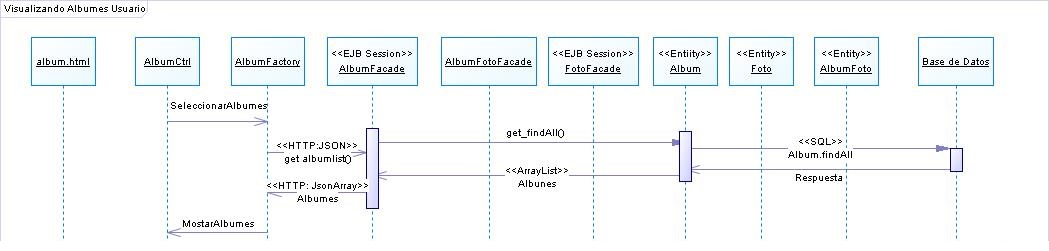
\includegraphics[width=16.5cm]{DiagramaSecuenciaAlbumesUsuarioParteA.jpg}
}

\figura{Diagrama de Secuencia: Visualizando Álbumes Usuario.}{
	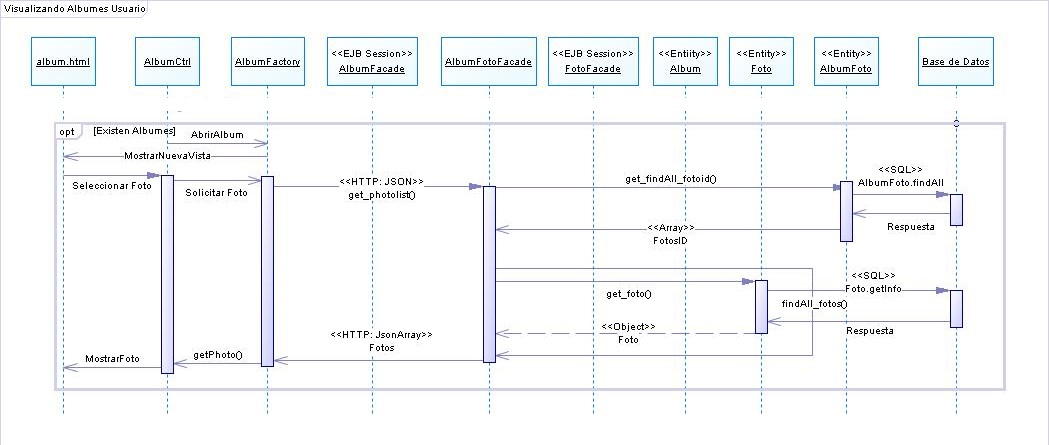
\includegraphics[width=16.5cm]{DiagramaSecuenciaAlbumesUsuarioParteB.jpg}
}

En este diagrama de secuencia se busca mostrar el comportamiento del sistema ante eventuales acciones por parte del usuario, en este caso el usuario se encuentra en primera instancia en la vista Álbumes, luego al cargar la página en el navegador se recibe la petición desde la vista y se procesa gracias a \textsl{angularJS} mediante los módulos \textsl{AlbumCtl} y \textsl{AlbumFactory} los cuales envían y contactan al \textsl{web service} mediante una petición HTTP esta petición la recibe el \textsl{EJB} correspondiente el cual procesa la consulta y entrega la información adecuada que en este caso es un \textsl{JSON} que contiene la información de las fotografías del usuario. Cabe destacar que este \textsl{JSON} se genera en primera instancia gracias a la comunicación realizada entre el \textsl{EJB} y el \textsl{entity} correspondiente a Álbum. Y de estos \textsl{entities} con la base de datos.  Luego en caso que existan álbumes en la base de datos se entregará la posibilidad al usuario de ver las fotografías contenidas en cada álbum. Realizando un proceso de comunicación similar al anterior pero extrayendo nueva información del sistema para cada fotografía perteneciente al álbum seleccionado. Cabe destacar que \textsl{angularJS} se encarga de el recambio de vista en caso de que existan álbumes y fotos en éstos.


%-------------------------------------------------------------------------------------
\capitulo{DICCIONARIO DE DATOS.}

A continuación, se presenta el diccionario de datos, que contendrá y detallará los atributos correspondientes de la base de datos.

\begin{enumerate}
\item \textbf{ALBUM}: las funcionalidades que se asocian a el agrupamiento de fotografías bajo un nombre y descripción, además se tiene que un álbum pertenece a un usuario.

	\begin{enumerate}
	\item \textbf{ID\_ALBUM}: toda tabla posee un identificador, este atributo representa esto.
	\item \textbf{ID\_USUARIO}: como se mencionó anteriormente, un álbum pertenece a un usuario, por lo que este usuario es identificado con este atributo.
	\item \textbf{NOMBRE}: este atributo es la representación del nombre del álbum, este atributo es otorgado por el usuario que crea éste.
	\item \textbf{FECHA\_CREADO}: atributo que representa la creación del álbum en una fecha específica.
	\item \textbf{DESCRIPCION}: atributo que es ingresado por el usuario, donde el usuario puede o no describir el contenido del álbum, por ende este atributo puede ser NULL, es decir puede no existir.
	\item \textbf{CANT\_FOTO}: este atributo representa la cantidad numérica de las fotografías que están relacionadas al álbum, esta cantidad es modificada a través de un trigger mencionado posteriormente.
	\item \textbf{URLFOTOALBUM}: cada uno de los álbumes tendrá una foto asociada, aquí las fotografías serán descritas a través de una dirección para así ser posteriormente identificadas.
		\begin{itemize}
		\item \textbf{aumentarCantAlbums}: este es un \textsl{trigger}, por el cual se aumenta la cantidad de álbumes del usuario cada vez que se inserte un nuevo álbum de éste.
		\end{itemize}
	\end{enumerate}
	
\item \textbf{ALBUM\_FOTO}: tabla que es utilizada para relacionar una fotografía con un álbum correspondiente.

	\begin{enumerate}
	\item \textbf{ID\_ALBUM}: necesita identificar el álbum al que se va agregar una fotografía.
	\item \textbf{ID\_FOTO}: se necesita saber que fotografía será la que se va agregar al álbum es por esto que se identifica un identificador.
	\item \textbf{FECHA\_AGREGACION}: a modo de tener claridad y mantener un orden de las fotos con respecto al tiempo real.
		\begin{itemize}
		\item \textbf{aumentarCantFotoAlbums}: \textsl{trigger} que es utilizado para poder ir cambiando el atributo CANT\_FOTO del álbum, cada vez que se agregue una relación de una fotografía con un álbum. 
		\end{itemize}
	\end{enumerate}

\item \textbf{ALBUM\_PERMISO}: tabla que se utiliza para poder relacionar un permiso con un álbum, pensando en que un álbum posee un permiso correspondiente que puede ser elegido por el usuario.

	\begin{enumerate}
	\item \textbf{ID\_ALBUM}: se necesita identificar el álbum al que se le agrega el permiso correspondiente.
	\item \textbf{ID\_PERMISO}: se necesita tener claro cuál es el permiso que se le va a asignar al álbum correspondiente.
	\end{enumerate}
	
\item \textbf{CAMARA}: como se sabe se van a necesitar cierta información de cámaras, para así ser relacionadas con una fotografía, como a la vez también proveer un análisis de las cámaras más utilizadas en la aplicación. 

	\begin{enumerate}
	\item \textbf{ID\_CAMARA}: se necesita poder identificar las cámaras, para poder evitar que si se quiere acceder a una cámara solo esta tenga el mismo identificador.
	\item \textbf{MEGAPIXELES}: una cámara posee una calidad de imagen, la cual es evaluada en megapíxeles.
	\item \textbf{ZOOM}: las cámara poseen cierto acercamiento máximo que pueden realizar, para esto se identifica un zoom que posee una cámara.
	\item \textbf{URL\_FOTO\_CAMARA}: se desea mostrar una imagen de la cámara para el análisis de éstas, es por esto que se debe tener una dirección asociada a esta imagen.
	\item \textbf{NOMBRE}: toda cámara posee un nombre para ser identificada, es por esto que esta la existencia de este atributo.
	\item \textbf{MODELO}: cada una de las cámaras poseen distintos modelos, es por esto que se pueden clasificar por un modelo.
	\item \textbf{CANT\_FOTOS}: se llevará la cuenta de cuantas fotografías son relacionadas con una cámara, esto para lograr realizar un análisis de éstas.
	\end{enumerate}
	
\item \textbf{CLASIFICACION}: tabla pensada en la utilización de WEKA, es por esto que se deja el espacio pensando en que en nuestro grupo tendremos que recibir un clasificador.

	\begin{enumerate}
	\item \textbf{ID\_CLASIFICACION}: se necesita identificar una clasificación correspondiente, es por esto que está la existencia de este atributo.
	\item \textbf{NOMBRE\_CLAS}: pensando en que existirá una etiqueta correspondiente para cada clasificación, es decir, este atributo tendrá el nombre de los tres tipos de clasificación, NEUTRA, POSITIVA o NEGATIVA.
	\end{enumerate}
	
\item \textbf{COMENTARIO\_ALBUM}: tabla utilizada para relacionar un comentario con un álbum, cabe mencionar que este está para el caso de \textsl{bonus}, es decir, solo está pensado en el caso de que alcance el tiempo para implementarlo, es utilizado para la existencia de comentarios a un álbum.

	\begin{enumerate}
	\item \textbf{ID\_COMENTARIO\_ALB}: se necesita identificar la relación que tendrá el álbum con el comentario.
	\item \textbf{ID\_ALBUM}: se necesita identificar el álbum con el cual está relacionado el comentario correspondiente.
	\item \textbf{ID\_CLASIFICACION}: se necesita identificar una clasificación correspondiente del comentario que existe en el álbum.
	\item \textbf{ID\_USUARIO}: se necesita identificar el usuario que realiza el comentario correspondiente que se está relacionando.
	\item \textbf{COMENTARIO\_ALB}: se almacena el comentario realizado al álbum correspondiente.
	\item \textbf{FECHA\_COMENTARIO}: se almacena una fecha correspondiente de cuando fue realizado el comentario.
	\end{enumerate}
	
\item \textbf{COMENTARIO\_FOTO}: cada foto tendrá comentarios asociados, es por esto que existe esta tabla, la cual contendrá el comentario y el usuario que realiza el comentario.

	\begin{enumerate}
	\item \textbf{ID\_COMENTARIO\_FOTO}: se debe identificar el comentario en la foto, es por esto la existencia de este atributo.
	\item \textbf{ID\_FOTO}: se necesita identificar la fotografía que posee este comentario.
	\item \textbf{ID\_CLASIFICACION}: pensando en la implementación de WEKA, se utiliza el identificador de la clasificación que posee el comentario.
	\item \textbf{ID\_USUARIO}: se necesita saber quién es el usuario que realiza el comentario en la fotografía correspondiente.
	\item \textbf{COMENTARIO\_FOTO}: se almacena el comentario correspondiente que se realiza.
	\item \textbf{FECHA\_COMENTARIO\_FOTO}: para manejar el tiempo de la realización del comentario correspondiente.
	
		\begin{itemize}
		\item \textbf{aumentarCantCom}: \textsl{trigger} utilizado para que cada vez que se agregue un comentario a una fotografía se aumente el contador de comentarios con la foto correspondiente.
		\end{itemize}
	\end{enumerate}
	
\item \textbf{ETIQUETA}: tabla que representa una referencia de un usuario en una fotografía.

	\begin{enumerate}
	\item \textbf{ID\_USUARIO}: se necesita tener asociado con el identificador del usuario para que este sea referenciado.
	\item \textbf{ID\_FOTO}: se necesita saber en qué fotografía será referenciado el usuario correspondiente.
	\end{enumerate}
	
\item \textbf{EVENTO}: tabla correspondiente a los eventos recientes, es decir, será utilizada para identificar las actividades recientes que se irán realizando en el sistema.

	\begin{enumerate}
	\item \textbf{ID\_EVENTO}: se necesita poder identificar los eventos para poder ser utilizados. 
	\item \textbf{FECHA\_EVENTO}: se necesita mantener un registro de la fecha en que ocurre este evento para así solo mantener los recientes.
	\item \textbf{ID\_USUARIO}: se necesita saber el usuario involucrado en el evento es por esto que se debe almacenar el ID de éste.
	\item \textbf{DESCRIPCION}: cada uno de los eventos posee una descripción correspondiente de lo que se hizo, es por esto que se tiene este atributo.
	\item \textbf{URL\_EVENTO}: para saber una dirección de una fotografía que está asociado el evento.
	\item \textbf{ID\_FOTO}: finalmente se necesita saber que fotografía es la que posee el evento asociado, es decir, si se comentó una foto se necesita saber que fotografía fue.
	\end{enumerate}
	
\item \textbf{FAVORITO\_ALBUM}: tabla que es utilizada para el caso en que se implemente el bonus comentado anteriormente, donde se puede establecer como favorito un álbum.

	\begin{enumerate}
	\item \textbf{FECHA\_FAV\_ALB}: en este atributo se desea almacenar la fecha en que se realizó el favorito del álbum.
	\item \textbf{ID\_USUARIO}: para llevar un manejo de quien realizó el favorito se necesita identificar el usuario a través de su ID.
	\item \textbf{ID\_ALBUM}: para ir manejando quien es el que posee el favorito, se necesita manejar el ID del álbum correspondiente.
	\end{enumerate}

\item \textbf{FAVORITO\_FOTO}: tabla utilizada para manejar el favorito de una fotografía.

	\begin{enumerate}
	\item \textbf{FECHA\_FAV\_FOTO}: se necesita establecer el tiempo en que se hizo favorita la fotografía.
	\item \textbf{ID\_USUARIO}: se identifica el usuario que le puso favorito a la fotografía correspondiente.
	\item \textbf{ID\_FOTO}: se identifica la fotografía a la cual se le asignó el favorito correspondiente.
	
		\begin{itemize}
		\item \textbf{aumentarCantFavFoto}: \textsl{trigger} utilizado para aumentar la cantidad de favoritos en una fotografía.
		\end{itemize}
	\end{enumerate}

\item \textbf{FOTO}: tabla que es utiizada para manejar toda la información que debe poseer una fotografía, esta tabla es considerada el núcleo de la base de datos, debido a que esta es la que será más utilizada y todas las demás se manejan alrededor de ésta.

	\begin{enumerate}
	\item \textbf{ID\_FOTO}: cada fotografía será manejada con un identificador, el cual no se puede repetir entre fotografías, es por esto que será auto-incrementable.
	\item \textbf{ID\_CAMARA}: si se necesita manejar la información de que cámara es la que realizó la fotografía se necesita identificar qué cámara.
	\item \textbf{ID\_USUARIO}: cada fotografía está asociada a un usuario, es por esto que se debe manejar quien es el usuario a través de su ID.
	\item \textbf{FECHA\_CARGA}: se necesita saber en qué fecha se subió la fotografía, para así manejar el tema de las fotografías recientes.
	\item \textbf{FECHA\_TOMADA}: se sabrá además de la cámara la fecha en que fue tomada, eso sí  la cámara puede establecerlo.
	\item \textbf{VISTAS}: se manejará la cantidad de visitas que tiene cada fotografía en el sistema.
	\item \textbf{TITULO}: cada fotografía tendrá un título que será ingresada por el usuario que realizó la carga de ésta.
	\item \textbf{DESCRIPCION}: así como un título además la fotografía posee una descripción que también será cargada por el usuario.
	\item \textbf{CANT\_FAVOR}: Cada fotografía tendrá cierta cantidad de favoritos, esto será manejado a través de un \textsl{trigger}.
	\item \textbf{URL}: cada fotografía tendrá asociada una dirección para la ubicación de esta y así poder visualizarla.
	\item \textbf{FORMATO}: cada una de las fotografías pueden manejar un formato diferente, el cual por ejemplo puede ser JPEG.
	\item \textbf{PUNTO\_LUGAR}: como se desea manejar una ubicación si el usuario lo desea se almacenará un punto en particular de ubicación de la fotografía.
	\item \textbf{CANT\_COM}: se maneja la cantidad de comentarios que posee la fotografía, esto es manejado a través de un \textsl{trigger}.
	
		\begin{itemize}
		\item \textbf{aumentarCantFotoUsuario}: \textsl{trigger} utilizado para aumentar la cantidad de fotografías que posee un usuario, cada vez que su id corresponda con el de la fotografía se aumenta el contador.
		\end{itemize}
	\end{enumerate}

\item \textbf{FOTO\_PERMISO}: cada una de las fotografías posee un permiso correspondiente que el usuario le otorga dentro de los posibles.

	\begin{enumerate}
	\item \textbf{ID\_FOTO}: para otorgar un permiso, se debe identificar la fotografía a la cual se está asignando un permiso.
	\item \textbf{ID\_PERMISO}: para asignar un permiso se debe identificar el permiso correspondiente de la tabla permisos.
	\end{enumerate}

\item \textbf{LUGAR}: para le manejo de los mapas se tienen asociado una tabla que contendrá los lugares posibles de búsqueda.

	\begin{enumerate}
	\item \textbf{ID\_LUGAR}: identificador del lugar que se desea buscar.
	\item \textbf{POLYGON}: cada uno de los lugares será representado con un polígono correspondiente, el cual consta de ciertas coordenadas.
	\item \textbf{NOMBRE}: cada uno de los lugares representados en el mapa para la búsqueda poseen un nombre, como por ejemplo Santiago.
	\end{enumerate}

\item \textbf{PERMISO}: tabla utilizada para almacenar los tipos de permisos posibles que pueden tener las fotografías y si es posible los álbumes.

	\begin{enumerate}
	 \item \textbf{ID\_PERMISO}: se tiene un identificador del permiso correspondiente.
	 \item \textbf{COMPARTIR}: booleano correspondiente para permitir compartir la fotografía o álbum.
	 \item \textbf{COMENTAR}: booleano correspondiente para permitir comentar la fotografía o álbum.
	 \item \textbf{DESCARGAR}: booleano correspondiente para permitir descargar la fotografía o álbum.
	 \end{enumerate}
	 
\item \textbf{TAG}: como se desea la implementación de Tag, se necesita una tabla que posee algunos de éstos.

	\begin{enumerate}
	 \item \textbf{ID\_TAG}: se debe identificar cada uno de los posibles tags que posee la aplicación.
	 \item \textbf{NOMBRE\_TAG}: cada uno de éstos tendrá un nombre correspondiente al tag en sí.
	 \end{enumerate} 

\item \textbf{TAG\_FOTO}: tabla utilizada para asociar un tag a una fotografía en particular.

	\begin{enumerate}
	\item \textbf{ID\_TAG}: se debe identificar el tag que se está utilizando.
	\item \textbf{ID\_FOTO}: se debe determinar en qué fotografía se está otorgando el tag correspondiente.
	\end{enumerate}
	
\item \textbf{TAG\_USUARIO}: tabla utilizada para relacionar un tag con un usuario en particular que utiliza este tag.

	\begin{enumerate}
	\item \textbf{ID\_USUARIO}: se necesita identificar el usuario que hizo la utilización del tag.
	\item \textbf{ID\_TAG}: se necesita identificar el tag correspondiente.
	\end{enumerate}
	
\item \textbf{USUARIO}: se tiene una tabla correspondiente a todos los usuario que van a estar en el sistema.

	\begin{enumerate}
	\item \textbf{ID\_USUARIO}: se necesita identificar con un ID diferente a cada uno de estos usuarios.
	\item \textbf{ALIAS}: se tiene un nombre de usuario que posee cada uno de estos, el cual debe ser diferente al de todos.
	\item \textbf{NOMBREREAL}: se debe almacenar el nombre real del usuario.
	\item \textbf{CONTRASEÑA}: cada uno de los usuarios posee una contraseña correspondiente para su alias.
	\item \textbf{FECHA\_CREACION}: se almacena la fecha en que el usuario fue ingresado en el sistema.
	\item \textbf{APELLIDO}: usuario en el momento de registro debe almacenar su apellido.
	\item \textbf{CORREO}: cada uno de los usuarios debe ingresar a través de su correo al sistema, si que debe ser almacenado este.
	\item \textbf{CANT\_FOTOS}: cada usuario posee una cantidad de fotos subidas en el sistema, para esta funcionalidad se utiliza un \textsl{trigger} correspondiente.
	\item \textbf{CANT\_ALBUM}: cada usuario posee una cantidad de álbumes creados en el sistema.
	\item \textbf{CANT\_SEGUIDORES}: cada usuario puede ser seguido por otros usuarios, es por esto que se maneja la cantidad de seguidores que posee.
	\item \textbf{CANT\_SEGUIDOS}: además de cada uno de los seguidores se posee a cuantos usuarios sigue éste.
	\item \textbf{URL\_PERFIL}: se necesita la dirección de la imagen en el sistema para poder asociarle una foto de perfil.
	\item \textbf{URL\_AVATAR}: cada uno de los usuarios posee una fotografía de avatar, es por esto que se maneja una dirección de la fotografía.
	\item \textbf{DESCRIPCION}: cada uno de los usuarios puede redactar una descripción correspondiente a ellos.
	\end{enumerate}
	
\item \textbf{USUARIO\_USUARIO}: como se menciona con anterioridad, los usuarios pueden seguirse esta tabla manejará esta información.

	\begin{enumerate}
	\item \textbf{ID\_USUARIO}: identificador del usuario que está siguiendo a otro usuario.
	\item \textbf{ID\_USUARIOFOLLOW}: identificador del usuario al cual se va a seguir.
	\item \textbf{FECHA\_SEGUIDOS}: se maneja la fecha en que se empieza a seguir a otro usuario.
	
		\begin{itemize}
		\item \textbf{aumentarCantSeguidores}: \textsl{trigger} para modificar cada vez que corresponda la cantidad de seguidores de un usuario que correponda.
		\item \textbf{aumentarCantSeguidos}: \textsl{trigger} para modificar cada vez que corresponda la cantidad de seguidos de un usuario que corresponda.
		\end{itemize}
	\end{enumerate}

\end{enumerate}

%-------------------------------------------------------------------------------------
\capitulo{DETALLE DE CASOS DE USO IMPLEMENTADOS.}

Si bien se planificó dentro de los Casos de Uso la implementación de la vista de fotografías y álbumes, se decidió comenzar en la implementación por una precondición necesaria para ambos Casos de Uso: El Inicio de Sesión y el Registro.

Tomando como base el Prototipo mostrado en entregas anteriores, se cambió el sistema de navegación por Rutas de \textsl{AngularJS}:

\figura{Implementación, pantalla principal.}{
	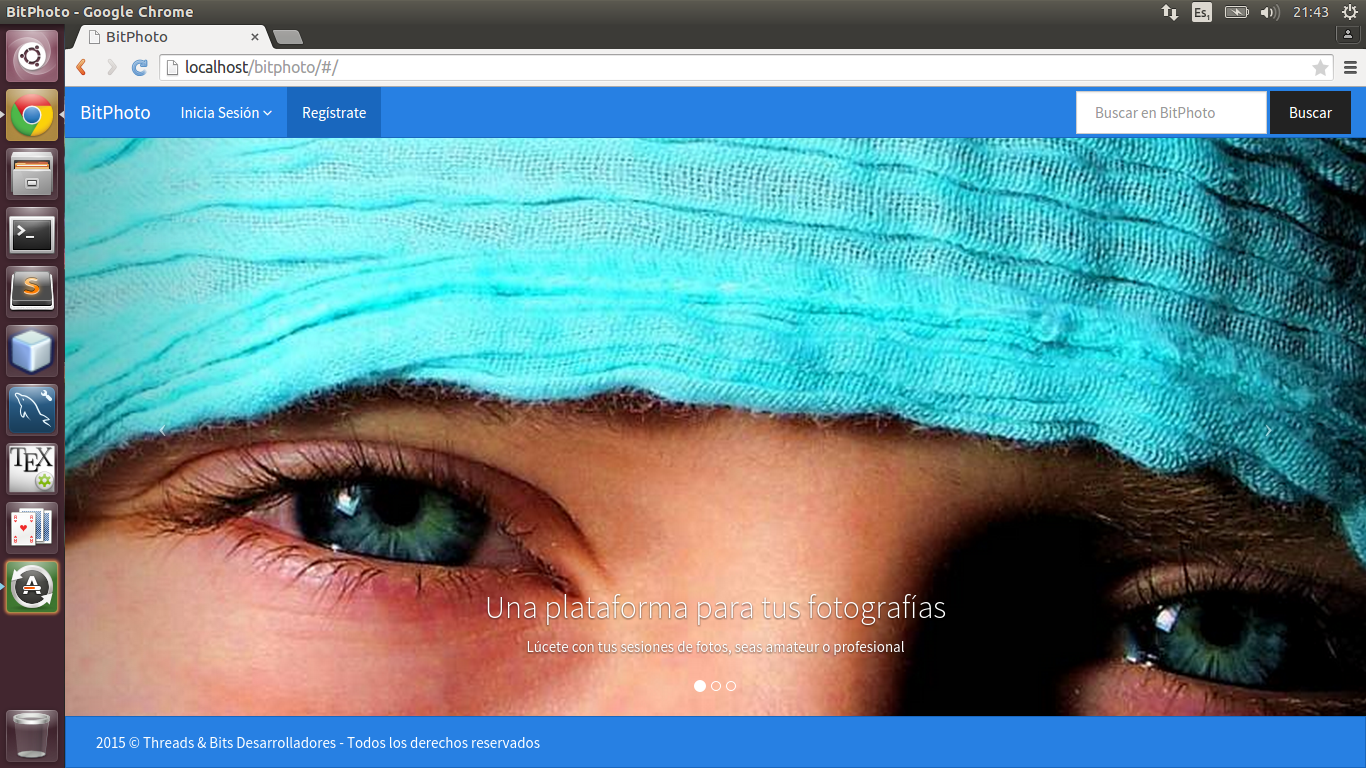
\includegraphics[width=16cm]{login1.png}
}

Si bien no es un cambio notorio en la vista como tal, el usar el módulo de navegación nativo de \textsl{AngularJS} permite cargar controladores en cualquier vista de la aplicación web.

Luego se procedió a implementar la validación de formularios potenciada por \textsl{AngularJS}, la cual permite verificar que los datos tengan contenido admisible por el campo en cuestión (por ejemplo, que una dirección de correo electrónico tenga una arroba).

\figura{Implementación registro.}{
	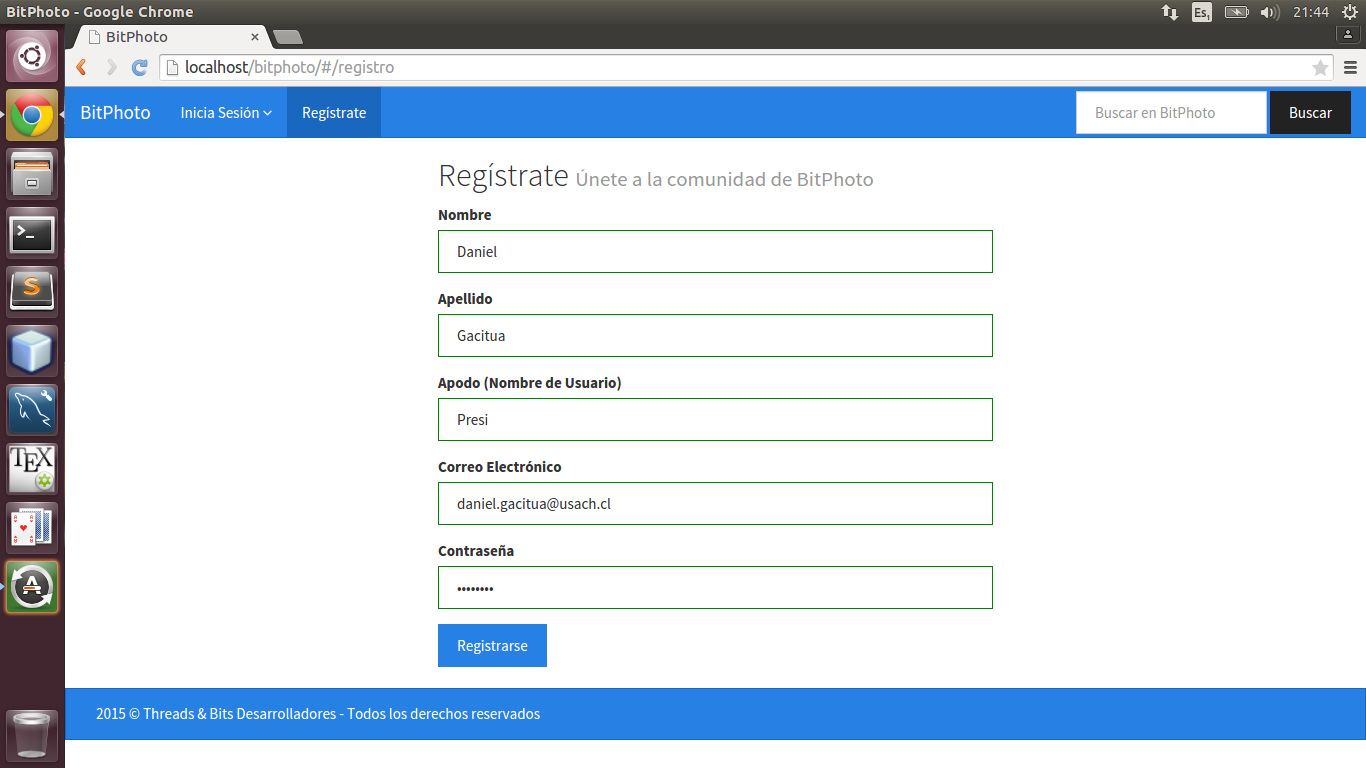
\includegraphics[width=16cm]{login2.png}
}

Con estos elementos terminados, se construyó el código de autenticación en \textsl{AngularJS} para el Inicio de Sesión y el Registro. Como aún no se ha podido realizar la integración de servicios \textsl{REST} con \textsl{JavaEE}, se implementó un servicio \textsl{REST} falso (basado en \textsl{LocalStorage}) para guardar los datos de registro.

\figura{Implementación login.}{
	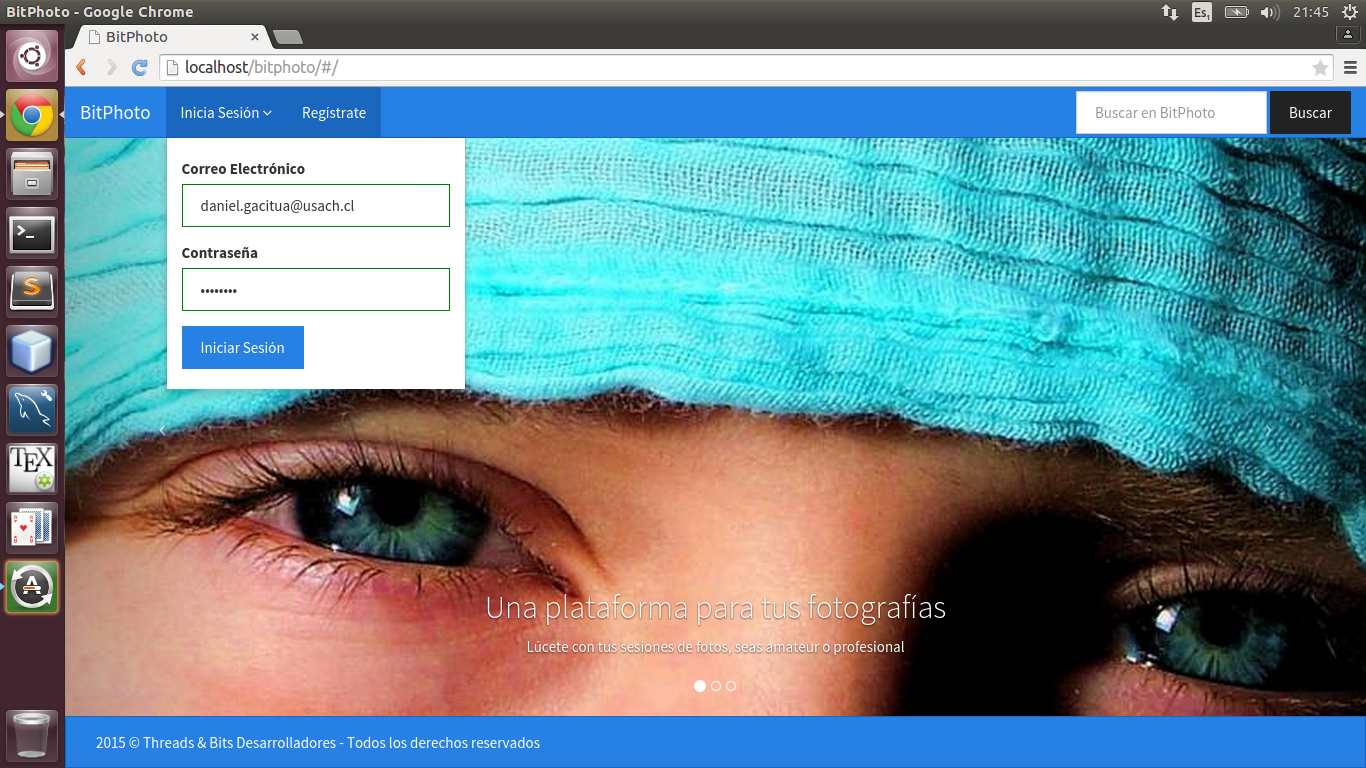
\includegraphics[width=16cm]{login3.png}
}

El sistema de autenticación actual tiene la facultad de crear \textsl{cookies} de navegador que permiten la persistencia de la sesión, y obtener datos adicionales y personalizados de cada usuario.

\figura{Implementación, subir fotografía.}{
	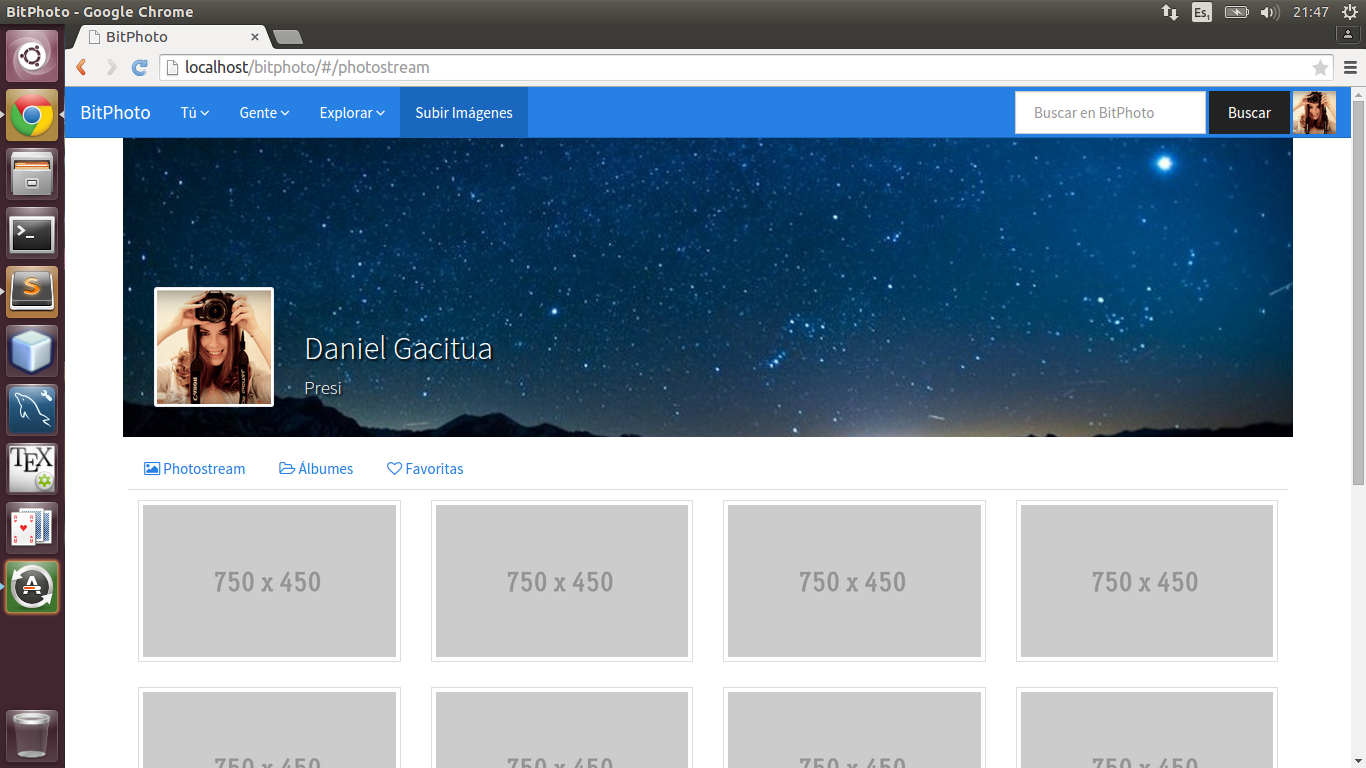
\includegraphics[width=16cm]{login4.png}
}

Las imágenes y otros elementos aún permanecen estáticos, y serán implementados en entregas posteriores, basados en la implementación recién mencionada.


%-------------------------------------------------------------------------------------
\capitulo{GESTIÓN DEL PROYECTO.}

\seccion{ORGANIZACIÓN DE REPOSITORIOS GIT.}
    
Para optimizar la creación de código, favorecer la correcta colaboración entre los integrantes y tener un versionamiento ordenado del código, se decide emplear a git como sistema de control de versiones, y usar GitHub como servidor remoto de git.\\

Cada miembro del grupo utiliza una cuenta de GitHub:

\begin{itemize}
	\item \textbf{Gerson Aguirre}: \textsl{https://github.com/GersonAguirre}
	\item \textbf{Max Chacón}: \textsl{https://github.com/nanochacon}
	\item \textbf{Daniel Gacitúa}: \textsl{https://github.com/GaciX}
	\item \textbf{Elías González}: \textsl{https://github.com/Elitos}
	\item \textbf{Nicolás Rozas}: \textsl{https://github.com/NicoRozas}
\end{itemize}

Se ha creado la organización “tbd2015” que aloja todos los repositorios del proyecto: \textsl{https://github.com/tbd2015}.\\

Dentro de la organización, se han creado diferentes repositorios para cada módulo del proyecto:

\begin{itemize}
	\item \textbf{InformesTBD}: Contiene los informes y presentaciones del proyecto. 
	\item \textbf{Prototipo}: Contiene el prototipo gráfico de la Aplicación Web.
	\item \textbf{BitPhoto}: Contiene el módulo principal del proyecto (en JavaEE).
	\item \textbf{BitPhoto-Mobile}: Contiene la aplicación para Android del proyecto.
	\item \textbf{BitPhoto-Search}: Contiene el motor de búsqueda (potenciado por Apache Lucene).
	\item \textbf{BitPhoto-Miner}: Contiene el módulo de análisis de sentimientos (potenciado por Weka).
	\item \textbf{BitPhoto-Web}: Contiene la aplicación web del proyecto (potenciado por Angular JS).
\end{itemize}

Cada miembro del grupo tendrá acceso a todos los repositorios para fomentar la colaboración. Cabe destacar que con un sistema modular de repositorios dentro de la organización ordena de mejor manera los aportes de cada miembro y ayuda a evitar el entorpecimiento al hacer commits de forma concurrente.

\newpage

\seccion{COMUNICACIÓN, AVANCES Y BURNDOWN.}

En la reunión de planificación realizada, se determinó que el segundo \textsl{Sprint} duraría hasta el 6 de Junio del 2015. Además se acordó las horas de trabajo diarias que se podían dedicar a la realización del proyecto, se estimó que cada integrante del grupo podría dedicar a lo máximo 1.5 hrs al dia para el proyecto. Luego se definieron las tareas para que estas se pudieran realizar en un tiempo cercano al de trabajo diario estimado, luego se estimó cada tarea en estar realizada.

Para la realización de la tercera entrega el grupo optó por varios canales de comunicación para manejar las relaciones entre los participantes, por lo tanto se determinaron distintas tecnologías para objetivos específicos, los canales usados para comunicarse entre el grupo fueron los siguientes:

\begin{itemize}
	\item Grupo \textbf{\textsl{WhatsApp}}, con el fin de conversar inmediatamente y de forma rápida temas relacionados con el proyecto, principalmente se utilizó para dudas cortas y compartir pequeñas opiniones del proyecto.
	\item Grupo \textbf{\textsl{Facebook}}, para registrar minutas, información relevante y noticias que afecten a todos los integrantes del grupo.
	\item Se creo una carpeta en \textbf{\textsl{Google Drive}}, para con el fin de compartir documentos referentes al informe, presentaciones, entre otras, correspondientes a la entrega de diseño arquitectural.  
	\item Se utilizó la aplicación \textbf{\textsl{Trello}} para organizar las partes que se debían realizar en la entrega, además esta aplicación permite organizar las partes del proyecto definiendo las tareas personalmente y los tiempos con los que fueron realizadas cada una de estas.
	\item Para controlar las versiones del informe y los prototipo de las vistas se utilizó la herramienta \textbf{\textsl{Git}} que permite controlar las versiones de estas dos partes del proyecto. Esta tecnología se utiliza para archivos de texto plano y para controlar las modificaciones que se le pueden realizar a éstos.
\end{itemize}

\newpage

A continuación se presentan las tareas definidas y las estimaciones. Las estimaciones se realizaron con la metodología Pocket Card, utilizando la siguiente escala de medidas 0 - 0.5- 1- 2- 3- 5- 8- 13- 21.


\figura{Tareas 1-21}{
	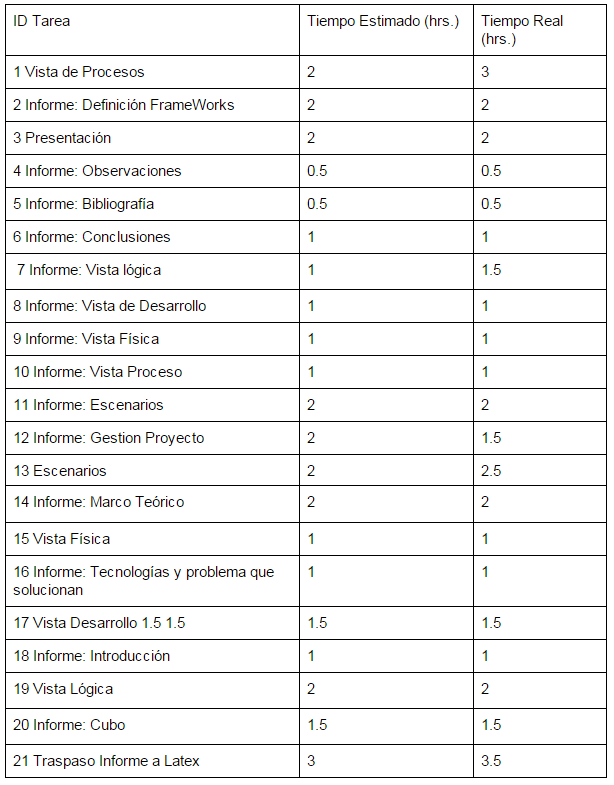
\includegraphics[width=15cm]{estimacionTareas1.png}
}


Ahora la cantidad estimada de peso por todas las tareas fue de 75 unidades de trabajo (trabajo realizado), Las unidades de trabajo real total fueron 92 (trabajo realizado), notar que los pesos totales reales trabajados superaron los pesos totales estimadas en 17 unidades de trabajo.  El margen de error fue relativamente alto ya que la escala para la estimación tomaba saltos demasiado grandes entre un peso y otro. El peso promedio por tarea fue de 7.08 unidades de trabajo.Otros datos que se obtiene al analizar lo anterior son:

\begin{itemize}
	\item Estimación Trabajo Diario Grupo: 7.5 
	\item Horas Disponibles en Sprint por cada integrante: 37.5 
	\item Horas Disponibles en Sprint del Grupo: 187.5 
	\item Trabajo por dia promedio ideal 2.59 
\end{itemize}

A continuación se presentan los gráficos \textsl{BurnDown} y \textsl{BurnUP} con el fin de señalar la forma en que se trabajó a lo largo del \textsl{Sprint}.


\figura{Gráfico Burnup}{
	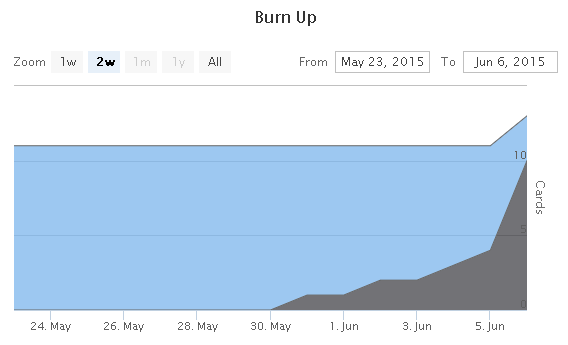
\includegraphics[width=15cm]{burnUp.png}
}

\newpage
\figura{Gráfico BurnDown}{
	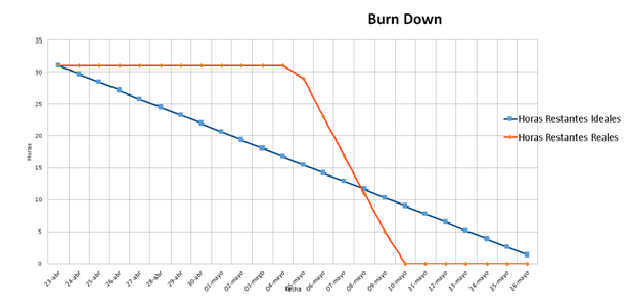
\includegraphics[width=15cm]{burnDown.png}
}

Como se aprecia en la imagen, se observa que en determinados periodos se trabajó una mayor cantidad, se alcanzó a realizar la mitad del trabajo estimado en 5 de Junio, esto sucede principalmente por la falta de atomicidad de las tareas y los procesos que lleva cada tarea, ya que pasa por un estado intermedio desde \textsl{estoy haciendo} a \textsl{finalizado} hay un estado de revisión donde los miembros del grupo se encargan de revisar el trabajo realizado por los otros compañeros del equipo. Luego desde el 30 de mayo en adelante se comenzó a trabajar con gran rapidez. Cabe destacar que los gráficos no se tocan ya que faltan tareas por concluir que fueron las tareas correspondientes a la implementación de los casos de uso.

Cabe destacar que para esta entrega se estimaron las tareas con \textsl{PokerPlaning} y se utilizó una plataforma para realizar en análisis de datos, denominada \textsl{ollertApp}, la cual facilita el análisis de manera directa con lo realizado en \textsl{trello}.


%-------------------------------------------------------------------------------------
\capitulo{OBSERVACIONES.}

En esta ocasión no se indicaron observaciones pertinentes al contenido del informe, sino mas bien consejos y sugerencias con respecto a la planificación, organización y trabajo en equipo.

%-------------------------------------------------------------------------------------
\capitulonn{CONCLUSIONES.}

Se puede finalizar este informe, acotando que esta entrega enseña un acercamiento más profundo y en detalle de la arquitectura de la aplicación \textsl{BitPhoto}. A través de los diagramas de clases y secuencia, junto con los casos de uso se permitió detallar la arquitectura de la aplicación para su posterior implementación. Se agregó también el diccionario de datos que incluye las definiciones básicas y terminología de los elementos de la plataforma.

Sobre la implementación de los Casos de Uso propuestos para esta entrega, no se pudieron llevar a cabo debido a la alta complejidad que suponía completarlos (además de la baja cantidad de horas-hombre disponibles para implementación), este alcance permitirá al grupo de desarrollo tener más experiencia a la hora de estimar a futuro las características a implementar en cada hito del proyecto, poniendo metas más realistas.

El resto de las tareas y objetivos pudo ser completado a cabalidad. Si bien las limitantes de tiempo propias de cada integrante del equipo impidieron tener una curva de \textsl{Burndown} ideal, el hecho de usar \textsl{Planning Poker} para la estimación de tareas y la organización colectiva a través de las vías de comunicación ya descritas favorecieron el cumplimiento del hito en los plazos indicados.



%-------------------------------------------------------------------------------------

\capitulonn{BIBLIOGRAFÍA.}

[1] Santiago Ceria. Ingeniería de Software I, Casos de Uso. 05/Junio/2015, de Universidad de Buenos Aires 
Sitio web: http://www-2.dc.uba.ar/materias/isoft1/2001\_2/apuntes/CasosDeUso.pdf


[2] Modelo de Clases. 05/Junio/2015, de Universidad de Chile 
Sitio web: http://users.dcc.uchile.cl/~psalinas/uml/modelo.html


\end{document}